%%%%%%%%%%%%%%%%%%%%%%%%%%%%%%%%%%%%%%%%%
% Beamer Presentation
% LaTeX Template
% Version 1.0 (10/11/12)
%
% This template has been downloaded from:
% http://www.LaTeXTemplates.com
%
% License:
% CC BY-NC-SA 3.0 (http://creativecommons.org/licenses/by-nc-sa/3.0/)
%
%%%%%%%%%%%%%%%%%%%%%%%%%%%%


%----------------------------------------------------------------------------------------
%	PACKAGES AND THEMES
%----------------------------------------------------------------------------------------

%\documentclass[10pt]{beamer}
\documentclass[aspectratio=169]{beamer}



\DeclareMathOperator*{\argmin}{arg\,min}


%%%%%%%%%%%%%

\usepackage{hyperref}


\newcommand{\bi}{\begin{itemize}}
\newcommand{\ei}{\end{itemize}}
\newcommand{\m}{\item}
\newcommand{\be}{\begin{enumerate}}
\newcommand{\ee}{\end{enumerate}}
\newcommand{\al}{\alert}
\newcommand{\ul}{\underline}


\mode<presentation> {

% The Beamer class comes with a number of default slide themes
% which change the colors and layouts of slides. Below this is a list
% of all the themes, uncomment each in turn to see what they look like.

%\usetheme{default}
%\usetheme{AnnArbor}
%\usetheme{Antibes}
%\usetheme{Bergen}
%\usetheme{Berkeley}
%\usetheme{Berlin}
%\usetheme{Boadilla}
%\usetheme{CambridgeUS}
%\usetheme{Copenhagen}
%\usetheme{Darmstadt}
%\usetheme{Dresden}
\usetheme{Frankfurt}
%\usetheme{Goettingen}
%\usetheme{Hannover}
%\usetheme{Ilmenau}
%\usetheme{JuanLesPins}
%\usetheme{Luebeck}
%\usetheme{Madrid}
%\usetheme{Malmoe}
%\usetheme{Marburg}
%\usetheme{Montpellier}
%\usetheme{PaloAlto}
%\usetheme{Pittsburgh}
%\usetheme{Rochester}
%\usetheme{Singapore}
%\usetheme{Szeged}
%\usetheme{Warsaw}

% As well as themes, the Beamer class has a number of color themes
% for any slide theme. Uncomment each of these in turn to see how it
% changes the colors of your current slide theme.

%\usecolortheme{albatross}
%\usecolortheme{beaver}
%\usecolortheme{beetle}
%\usecolortheme{crane}
%\usecolortheme{dolphin}
%\usecolortheme{dove}
%\usecolortheme{fly}
%\usecolortheme{lily}
%\usecolortheme{orchid}
%\usecolortheme{rose}
%\usecolortheme{seagull}
%\usecolortheme{seahorse}
%\usecolortheme{whale}
%\usecolortheme{wolverine}

%\setbeamertemplate{footline} % To remove the footer line in all slides uncomment this line
%\setbeamertemplate{footline}[page number] % To replace the footer line in all slides with a simple slide count uncomment this line

%\setbeamertemplate{navigation symbols}{} % To remove the navigation symbols from the bottom of all slides uncomment this line
}


%\setbeamertemplate{headline}
%{%
% \begin{beamercolorbox}{section in head/foot}
%\vskip1pt\insertnavigation{\textwidth}{}{}\vskip2pt
%  \end{beamercolorbox}
%}

\setbeamercolor{section in head/foot}{bg=lightgray} %set the top navigation bar background color
\setbeamertemplate{footline}[frame number] % set frame page number only
\usepackage{appendixnumberbeamer} % total will not include appendix frame numbers 

\beamertemplatenavigationsymbolsempty



\usepackage{graphicx} % Allows including images
% graphicx also allows for resizebox
% graphicx also allows for \scalebox
\usepackage{caption}
\usepackage{subcaption} % packgage for subcaption in subfigures
% The subfig and subcaption packages can not be used in cooperation with each other. Instead, you can usecaption package with subfig to add some flavor to the captions and subcaptions
\usepackage{bm} % make bold math symbols
\usefonttheme{professionalfonts}
%\usepackage{newtxtext,newtxmath} % for professional fond to load a Times Roman clone
\usepackage{tabularx} % extra features for tabular environment
\usepackage{booktabs} % Allows the use of \toprule, \midrule and \bottomrule in tables
\usepackage{adjustbox} % allows adjustbox
\usepackage{amsmath}  
\usepackage{amsfonts}
\usepackage{hyperref} % package for hyper link

% the following hypersetup makes link blue
\hypersetup{
  colorlinks   = true, %Colours links instead of ugly boxes
  urlcolor     = blue, %Colour for external hyperlinks
  linkcolor    = blue, %Colour of internal links
  citecolor   = blue %Colour of citations
}


\usepackage{float} % make the table H effective
\restylefloat{table}
\usepackage{color, colortbl}
\usepackage{booktabs} % package for tex professional table
\usepackage{mathtools} % package for \coloneqq
\usepackage{multirow} % multirow for intuition page.

% make pdf dark mode
%\usepackage{xcolor}
%\pagecolor[rgb]{0,0,0} %black
%\color[rgb]{0.5,0.5,0.5} %grey

\usepackage{pifont}% http://ctan.org/pkg/pifont
\newcommand{\cmark}{\ding{51}}%
\newcommand{\xmark}{\ding{55}}%



\usepackage{tikz} % graph in latex
\usetikzlibrary{positioning,arrows.meta} %tikz diagram
\usepackage{pgfplots}
\pgfplotsset{compat=newest} %this setting allow node to go to the correct place
\usepgfplotslibrary{fillbetween}

% use the tikz external library to cache tikz drawings
\usetikzlibrary{external}
\tikzexternalize[prefix=tikz/,optimize command away=\includepdf]


%\bibliography{bibliography}
%\usepackage[american]{babel}
%\usepackage{csquotes}
%\usepackage[style=apa]{biblatex}
%\DeclareLanguageMapping{american}{american-apa}
%\addbibresource{References.bib}

\usepackage{natbib} % package for citation


\usepackage{multicol}


%\usepackage{subfigure} % subfigure package
%\captionsetup[subfigure]{labelformat=empty}
% The subfig and subcaption packages can not be used in cooperation with each other. Instead, you can usecaption package with subfig to add some flavor to the captions and subcaptions

%\usepackage{natbib} % package for citation

% define a comment line that does nothing to hide content
\newcommand{\comment}[1]{}
\newcommand{\lnb}[1]{%
  \ln\left(#1\right)%
}
\renewcommand{\baselinestretch}{1.0} %  scales the default interline space to 1.0 its default value. 

% define a comment that can scale the equation 
\newcommand\scalemath[2]{\scalebox{#1}{\mbox{\ensuremath{\displaystyle #2}}}}

%----------------------------------------------------------------------------------------
%	TITLE PAGE
%----------------------------------------------------------------------------------------

\title[Payments]{\huge{Payments} \\
\vspace{6mm}
\small{MGT 4074 Fintech \& Crypto Tokens, Section A, Spring 2025}
} % The short title appears at the bottom of every slide, the full title is only on the title page


%\subtitle{Presentation to Shanghai International Studies University}


\author[Joseph Hall]{Joseph Hall} % Your name
\institute[GT]{Georgia Institute of Technology} % Your institution as it will appear on the bottom of every slide, may be shorthand to save space
 % Your institution for the title page
 % Your email address
 
\date{October 27, 2025} 
 % Date, can be changed to a custom date if without date



%---------------------------------------------------------------------------
\begin{document}

\newcolumntype{d}[1]{D{.}{.}{#1}}


\begin{frame}
\titlepage % Print the title page as the first slide
\end{frame}


%----------------------------------------------------------------------------------------

%	PRESENTATION SLIDES
%----------------------------------------------------------------------------------------

%-----------------------------------------------



%---------------------------------------------------------------------
%---------------------------------------------------------------------
%\section*{Introduction}
% When I comment the introduction section, fewer sections show up in navigation
%---------------------------------------------------------------------
%---------------------------------------------------------------------




\begin{frame}
\frametitle{Roadmap}
\tableofcontents
\end{frame}

%------------------------------------------------

%------------------------------------------------
% insert table of content before each section or subsection
%------------------------------------------------
\AtBeginSection[]
{
\begin{frame}
\frametitle{Roadmap}
%\tableofcontents[currentsection,currentsubsection]
\tableofcontents[currentsection]
\end{frame}
}

\AtBeginSubsection[]
{
\begin{frame}
\frametitle{Roadmap}
\tableofcontents[currentsection,currentsubsection]
%\tableofcontents[currentsection]
\end{frame}
}
%------------------------------------------------

\section{Final Project Rubrics}

\begin{frame}{Final Project Rubric: Smart Contracts}

The Rubric for Smart Contract Final Projects is: 

\bi 
\m \textbf{40 Points: Concept}
\bi 
\m Does this solution address a pressing need? 
\m Does this application play to the strengths of blockchain technology? 
\m Are the economics sound to the point where people will use it?
\ei 
\m \textbf{50 Points: Execution}
\bi 
\m Does the contract runs smoothly? 
\m Does your code clearly do what it says it does? 
\m Does it minimize gas costs? 
\ei 
\m \textbf{10 Points: Marketing}
\bi 
\m Is it presented attractively? 
\m Do I want to use it? 
\m Consider making a logo and/or catchy name for your project. 
\ei 
\ei 
    
\end{frame}


\begin{frame}{Final Project Rubric: Mini-Thesis}

The Rubric for Mini-Thesis Final Projects is: 

\bi
\m \textbf{40 Points: Strong Thesis Statement}
\bi 
\m Does the answer to this question have big implications for policy or management? 
\m Is the question controversial? 
\ei 
\m \textbf{50 Points: Empirical Support for Thesis Statement}
\bi 
\m Is the data source large, comprehensive, and suitable to answer the question? 
\m Do the data visualizations clearly support the thesis statement? 
\m Does your code clearly do what it says it does? 
\ei 
\m \textbf{10 Points: Presentation Quality}
\bi 
\m Is your thesis statement clearly and concisely articulated on the title slide? 
\m Are your data visualizations well-labeled and attractive? 
\m Does the presentation flow and hold the audience's attention? 
\ei 
\ei 
    
\end{frame}





\section{In the News}



\begin{frame}{US Treasury Stablecoins}


\begin{center}
    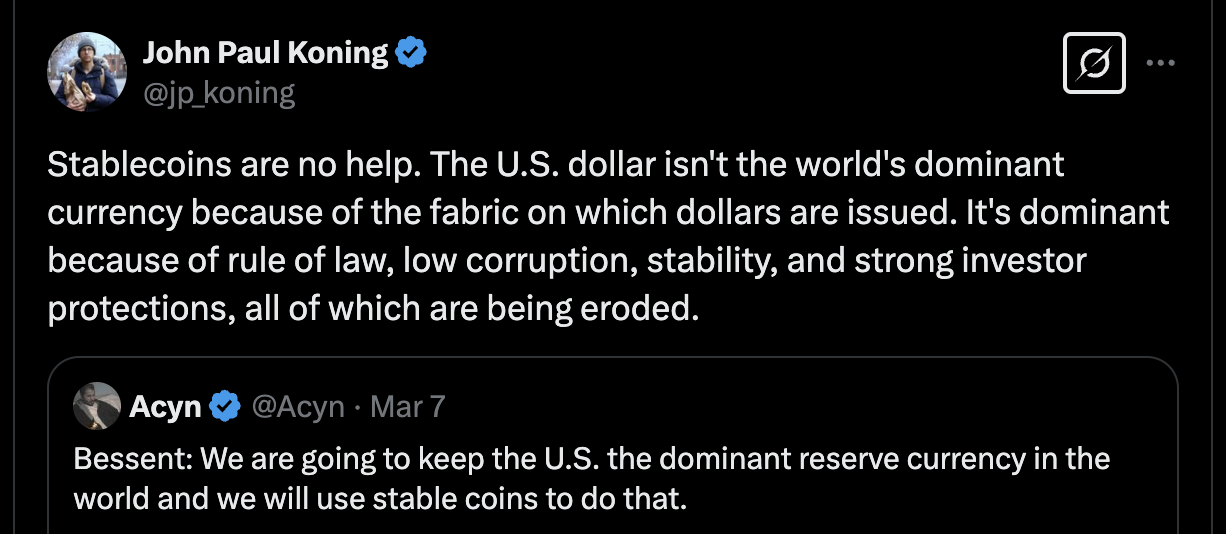
\includegraphics[width = .8\textwidth]{treasury_stablecoins.png}
\end{center}

\bi 
\m Does ``the fabric on which dollars are issued'' matter? \pause 
\m What about rule of law, low corruption, stability, and investor protections? \pause 
\m More coordination around dollars = more \emph{Seignorage} for the U.S.
\ei 
    
\end{frame}



\begin{frame}{U.S. Trade Deficit}


\begin{columns}
\begin{column}{0.5\textwidth}
    \begin{center}

   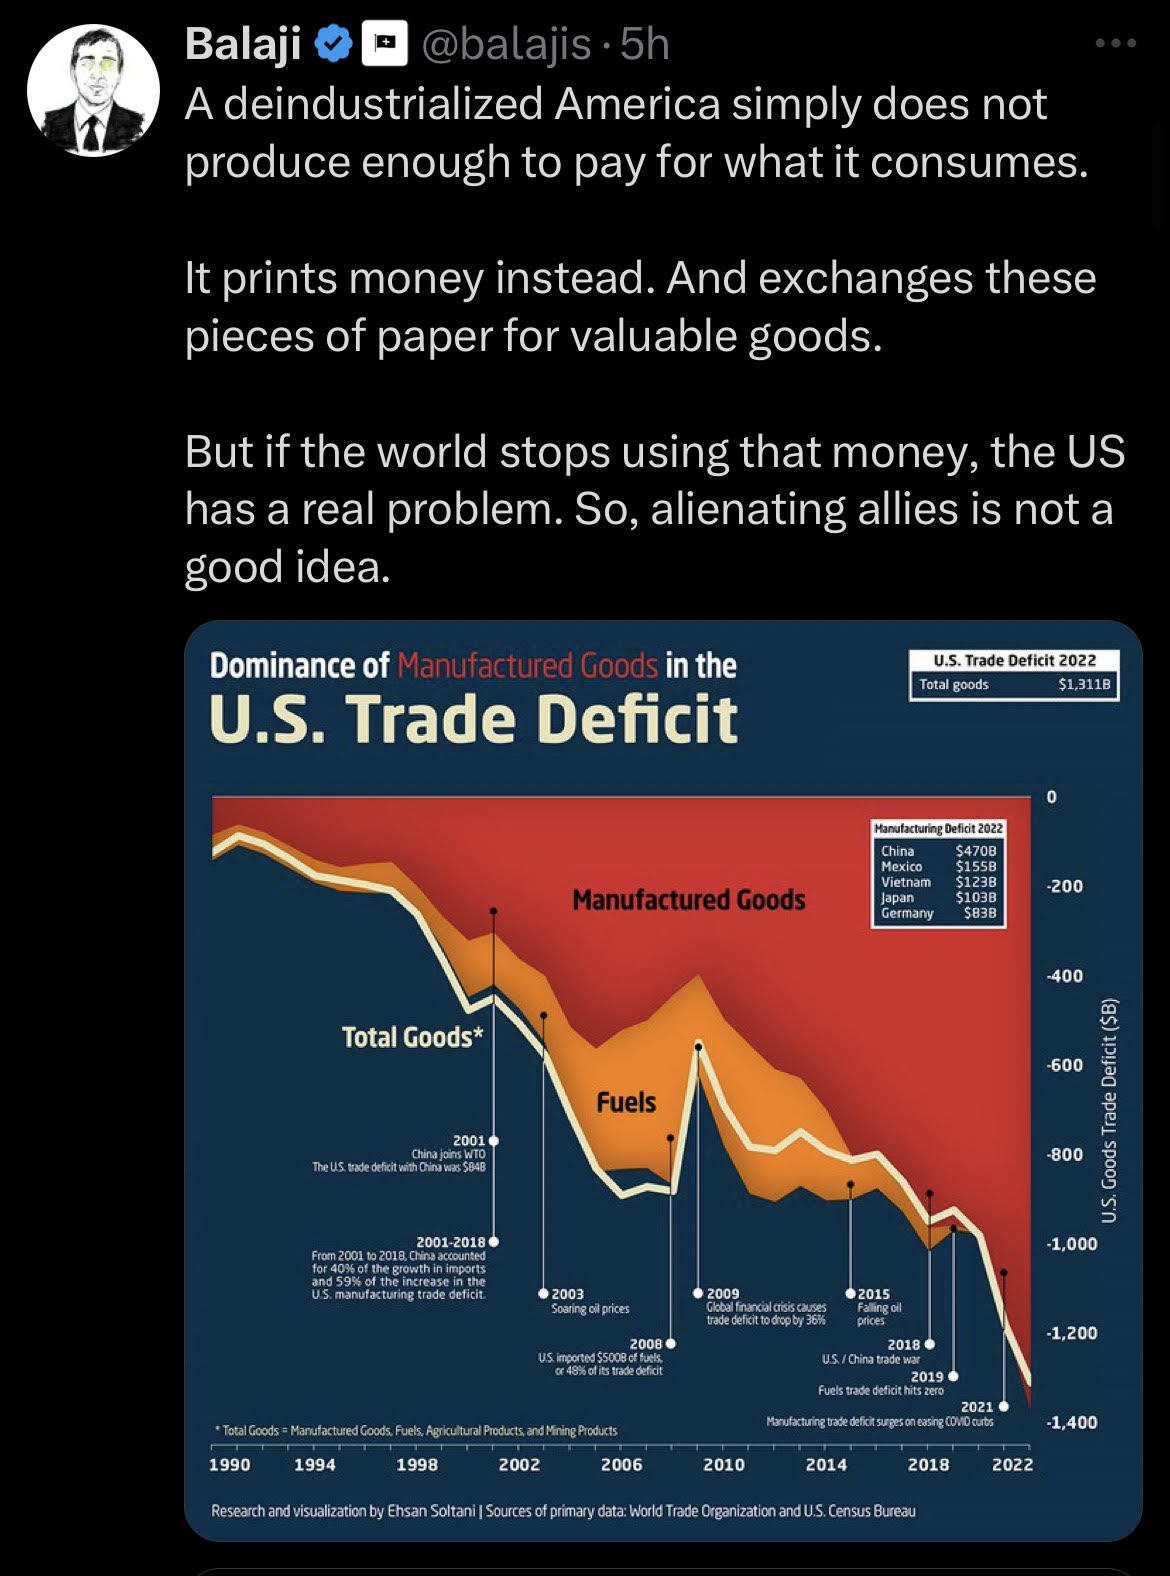
\includegraphics[width = .7\textwidth]{balaji.jpg}
     \end{center}

\end{column} \pause 
\begin{column}{0.5\textwidth}  
     Balaji is arguing the United States profits from \textbf{seignorage} because the U.S. dollar is a superior currency for international exchange to explain why the trade deficit is actually a good thing (he's right) \\ 
     \vfill \pause 
     The U.S. dollar has historically been a strong \textbf{store of value} and \textbf{medium of exchange} for international trade. Might that change? If it does, what consequences would that have? 
\end{column}
\end{columns}


\end{frame}

\begin{frame}{SP500 vs Bitcoin}

\begin{center}
    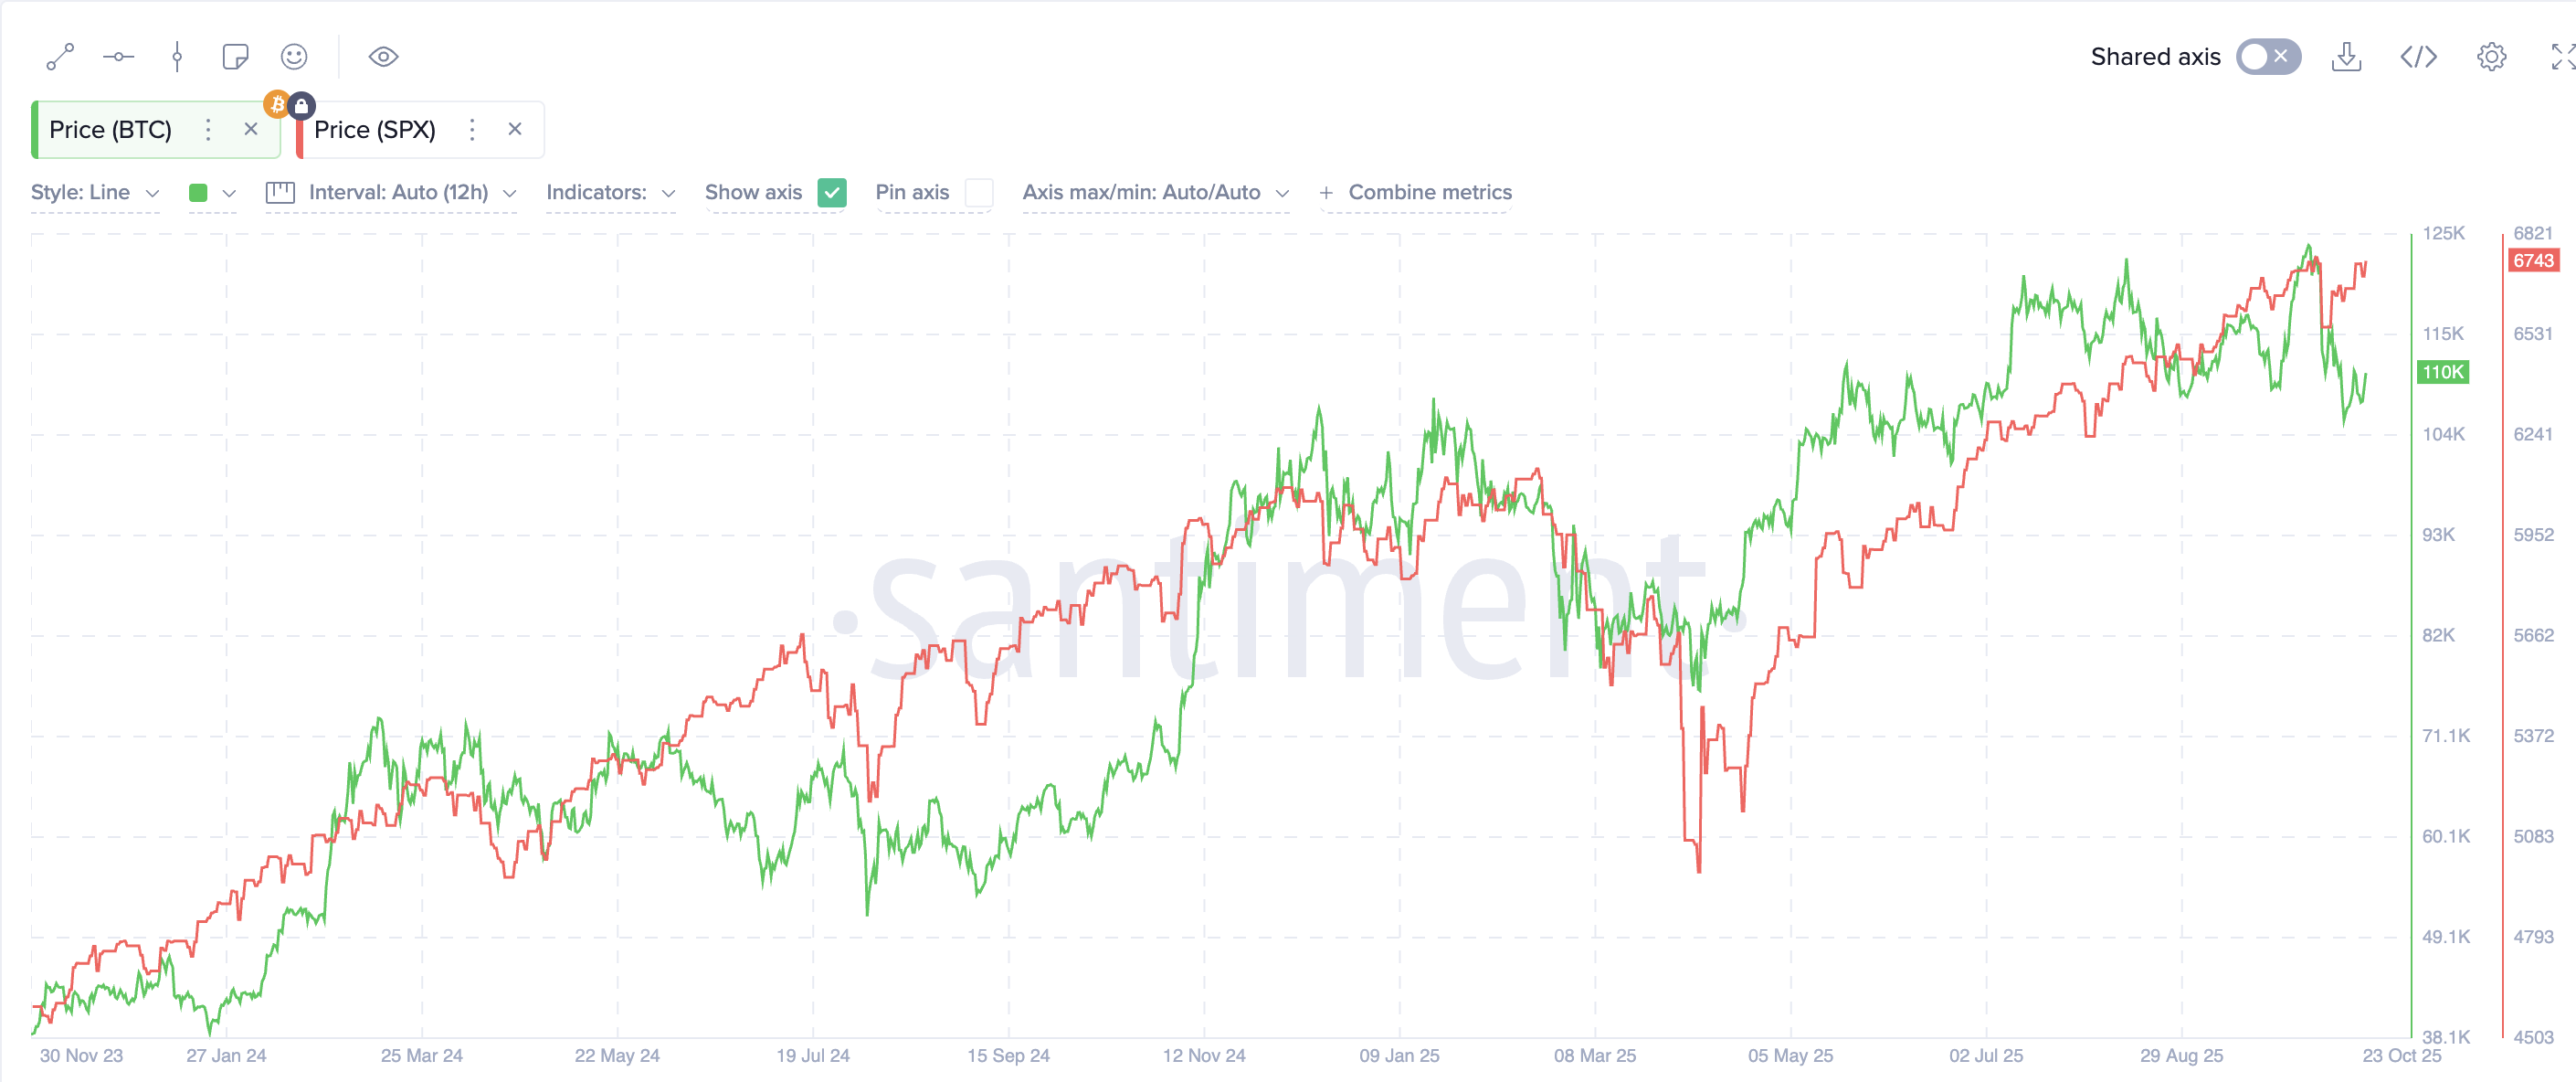
\includegraphics[width = .8\textwidth]{spx_btc.png}
\end{center}

\bi 
\m Why the close correlation? \pause Institutional investors who own both and buy/sell whole portfolio in unison? \pause 
\m Is Bitcoin a hedge against the stock market?
\ei 
    
\end{frame}




\section{Payments 101}


%------------------------------------------------

%\begin{frame}
%\frametitle{Payment Industry Jargon}


%\begin{itemize}
    %\item A \textbf{payment} is a transfer of money from one party to another %in exchange for goods and services.
    %\item \textbf{Methods of payment} include cash, debit, credit cards, and electronic fund transfers (EFTs).
    %\item A \textbf{money transfer} is the movement of money from one place to another. 
    %\item A \textbf{remittance} is a transfer of money to family abroad
    %\bi 
    %\m 
    %\ei 
    %\item A \textbf{cross-border payment} involves an foreign exchange (FX) transaction, where one currency is exchanged for another.
%\end{itemize}

	
%\end{frame} 
%----------------------------------------------------  




%------------------------------------------------

\begin{frame}
\frametitle{Payment Types and Fees}


\textbf{The \$2 trillion-dollar (McKinsey 2020 estimate) payments industry} has grown, fueled by e-commerce and the digital economy


Consumers and businesses face \textbf{many pain points} in payments and money transfer: \textbf{slow, non-transparent \& costly particularly when they cross national borders}.

\begin{itemize}
    \item A \textbf{bank wire} from one bank to another, for example, costs around \$20 and \$30 for outgoing transfer (2024) and \$10 for incoming transfer (2024) and takes several business days to arrive.
    \item Sending a \textbf{remittance} overseas may incur costs representing around 10\% of the proceeds (depending on sending and receiving counties) and could take weeks to arrive.
    \bi
    \m Latin America received \$145 Billion in remittances in 2021, approximately equal to all foreign direct investment (World Bank)
    \ei
    \item When sending a cross-border payment, the bank will deduct a \textbf{currency conversion fee} of up to 3\% and may delay the FX trade until it is advantageous for them.
\end{itemize}



\end{frame} 
%----------------------------------------------------  




%------------------------------------------------

\begin{frame}
\frametitle{Payment Fees by Banks by Area}


\vspace{-6mm}
%-----------------------------------------------
\begin{figure}[H]
    \resizebox{5.6in}{2.7in}{%
    %\resizebox{\textwidth}{!}{%
    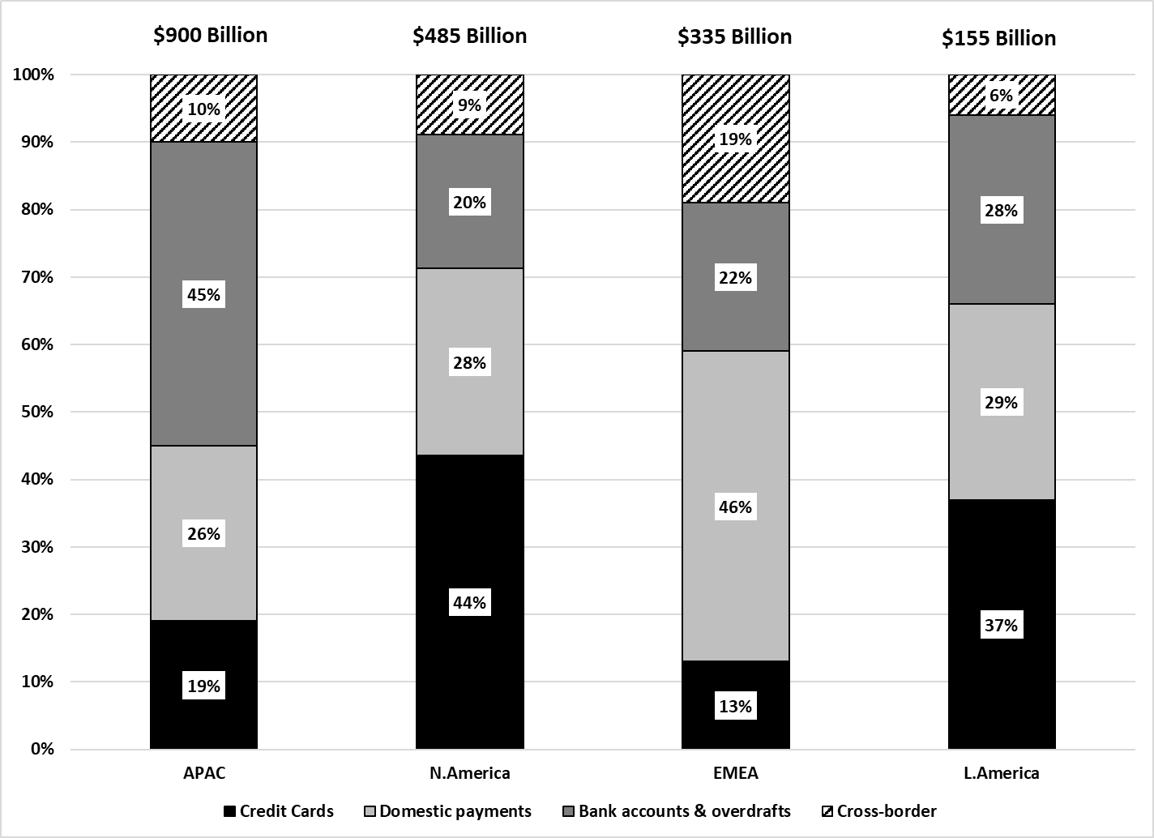
\includegraphics[]{pics/GlobalPaymentRevenue.png}
    } %end of resizebox
%-----------------------------------------------
% Figure setting: caption and label
%-----------------------------------------------
%\caption{Private Mortgages}
%\label{fig:ModelIntuition_Graphs}
\end{figure}
%-----------------------------------------------
\vspace{-2mm}


\end{frame} 
%----------------------------------------------------  



%------------------------------------------------

\begin{frame}
\frametitle{Payment Fees by Banks by Area}


\textbf{A \$2 Trillion Industry}:  \href{https://www.mckinsey.com/industries/financial-services/our-insights/the-2021-mckinsey-global-payments-report}{McKinsey} estimates it generates 40\% of bank revenues \\ 

Huge differences in payment industry revenue models by continent: 
\bi 
\m Credit cards are the dominant revenue stream in North America 
\m Europe, Middle East and African banks rely on domestic payment fees (mostly debit cards) 
\m Bank account fees and overdrafts are the dominant model in Asia-Pacific 
\ei 





\end{frame} 
%----------------------------------------------------  



\begin{frame}{Settlement}

A payment is \textbf{settled} when all balances are updated to reflect the payment
\bi 
\m Historically, banks have used \textbf{deferred net settlement}: 
\bi 
\m Each bank sends(/receives) \textbf{one} payment to the central clearinghouse at the end of each day equal to their \textbf{net outflows} \pause 
\m If sending a payment (e.g. moving a physical cart of gold) is expensive, this is dramatically cheaper: it does not scale at all with the number of payments, and scales \emph{linearly} with the number of banks! \pause 
\m DNS also solves a problem called \textbf{gridlock} (next slide)
\pause 
\m There is exposure to \textbf{counterparty risk}: a member can run away mid-day and default on their payables 
\ei 
\m \textbf{Real-time gross settlement} is the modern standard 
\bi 
\m Cost of digital payments on centralized systems approach zero
\m High gas fees in decentralized systems, and liquidity/gridlock problems for interbank transfers, remain good reasons to use DNS 
\ei 
\ei 
    
\end{frame}

\begin{frame}{Gridlock}

\textbf{Gridlock} can occur when desired trading volume is much higher than liquidity: 

\begin{center}
    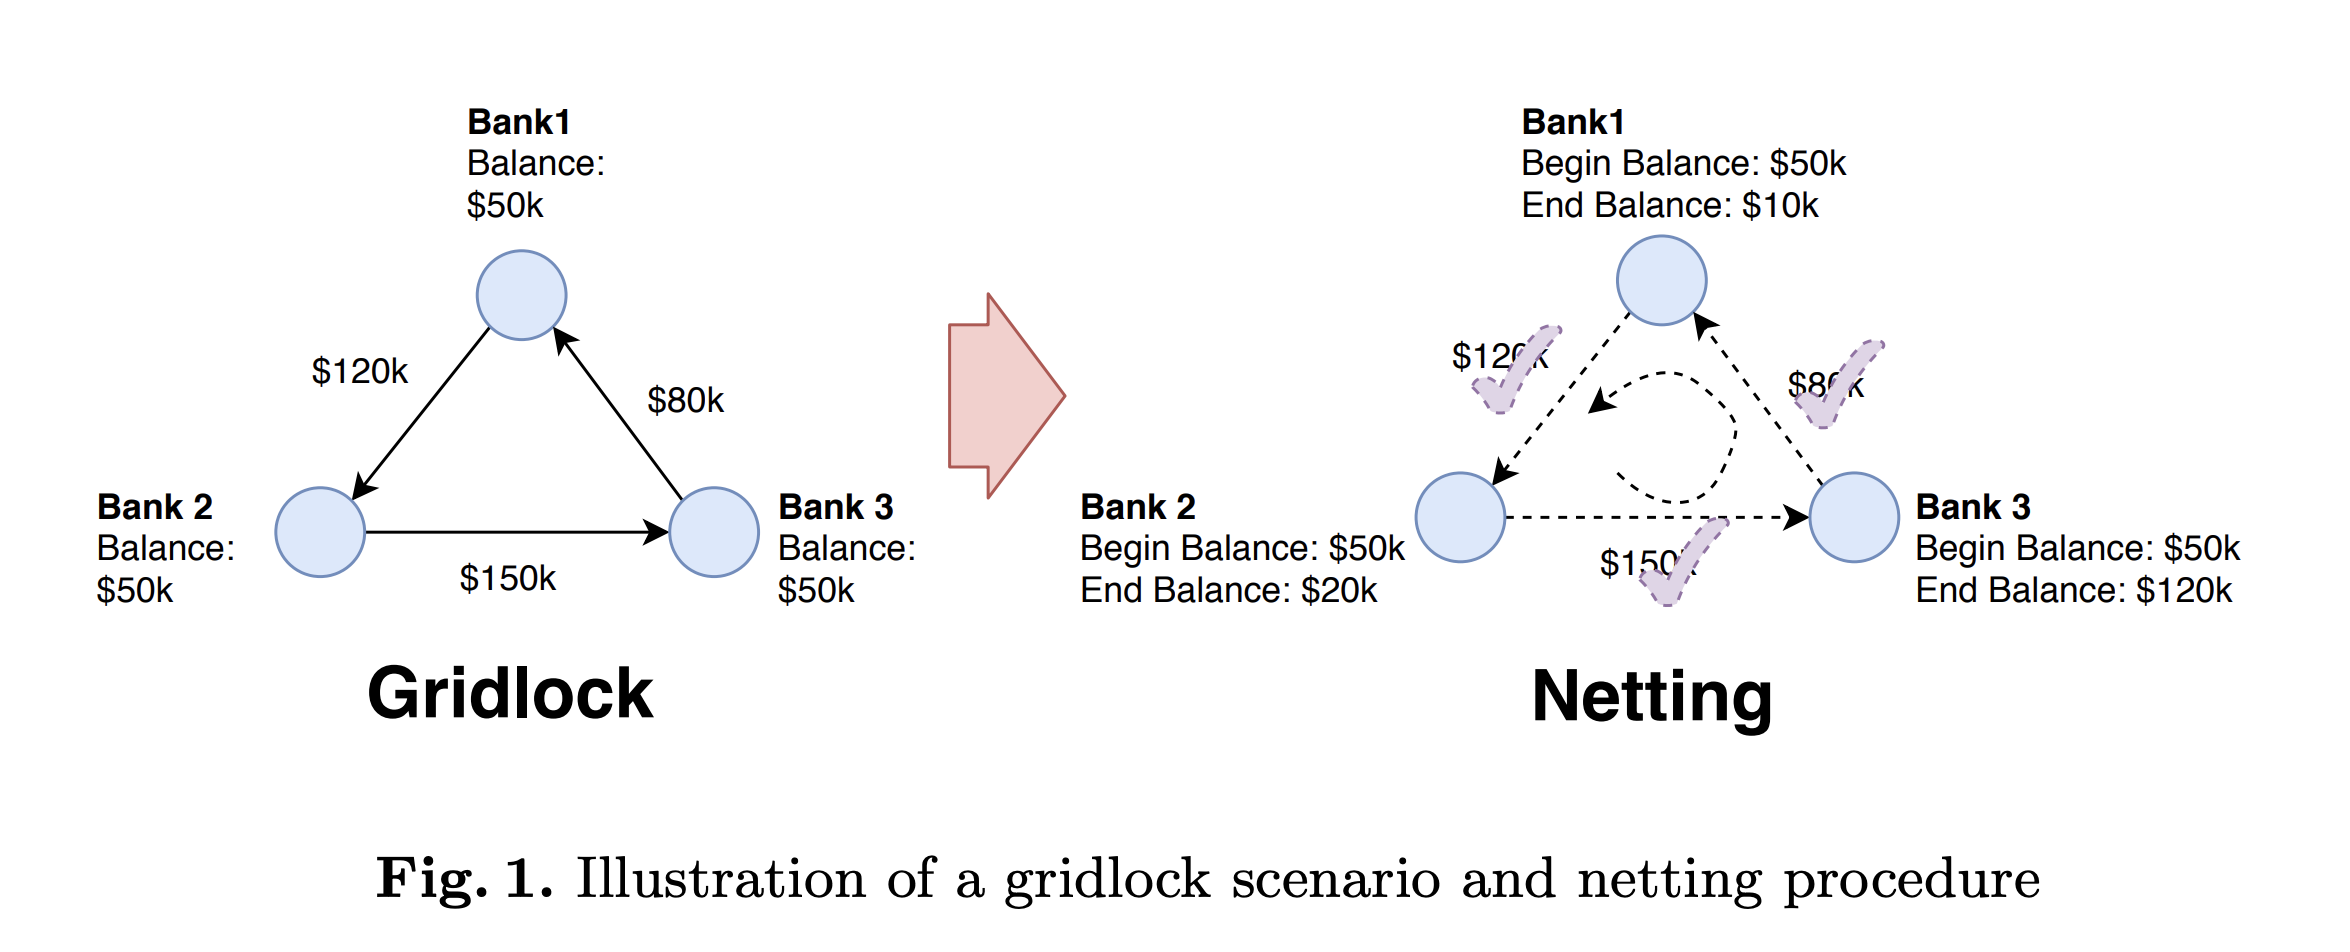
\includegraphics[width = \textwidth]{gridlock.png}
\end{center}

\href{https://www.ifca.ai/fc20/preproceedings/27.pdf}{Source: Cao et al (Ant \& IBM)}
    
\end{frame}


\begin{frame}{Gridlock}

Why does gridlock exist? 
\bi 
\m Banks prefer to hold as little liquidity as possible -- why? \pause 
\bi 
\m Would prefer to lend out money instead of keeping it in a vault 
\ei
\m ``Accident of history''/ sticky technology -- moving money between banks used to be technologically cumbersome 
\ei 
    
\end{frame}

%------------------------------------------------

\begin{frame}
\frametitle{Current Banking Payment Infrastructure}

\vspace{-2mm}
\textbf{The Payment Rails}: Electronic payments travel along a physical network of cables and wires connecting computers globally, known as the "payment rails".

\begin{itemize}
    \item \textbf{B2B payments use the Large value transfer system (LVTS)}: large sums of money and financial securities travel between banks, businesses \& government in 1 day or less, with many countries offering real-time gross settlement (RTGS).
    \begin{itemize}
        \item USA: Fedwire and CHIPS. Canada: Lynx. Europe: TARGET2.
    \end{itemize}
    \item \textbf{Consumer payments} via checks, credit \& debit use ``smaller rails'' with slower settlement: usually a few days. 
    \begin{itemize}
        \item USA: Automated Clearing House (ACH). Canada: ACSS
        \item Bo's Chase credit card on March 10th: transactions pending from March 7th
    \end{itemize}
\end{itemize}

\vspace{-3mm}
%-----------------------------------------------
\begin{figure}[H]
    \resizebox{3in}{1in}{%
    %\resizebox{\textwidth}{!}{%
    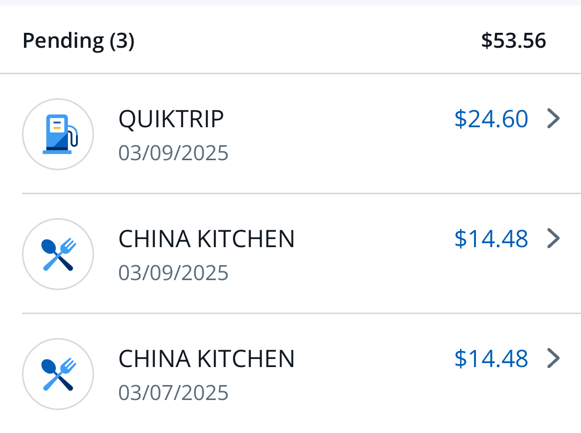
\includegraphics[]{pics/ChaseCrediCard_Takes3Days.png}
    } %end of resizebox
%-----------------------------------------------
% Figure setting: caption and label
%-----------------------------------------------
%\caption{Private Mortgages}
%\label{fig:ModelIntuition_Graphs}
\end{figure}
%-----------------------------------------------
\vspace{-2mm}


\end{frame} 
%----------------------------------------------------  




%------------------------------------------------

\begin{frame}
\frametitle{Payment Industry FinTech Companies}


\textbf{More \$1 billion fintech unicorns have been born in payments} than in any other area of financial services.

\smallskip  

Payments represent a vast opportunity for disruption.

\smallskip 
\begin{itemize}
    \item Fintechs are providing new payment methods, targeting \textbf{underserved customers}, \textbf{automating billing}, \textbf{reducing FX costs}, and \textbf{facilitating international remittances}.
    \smallskip 
    \item These innovations create trust, reduce frictions, and bring valuable services to unbanked populations.
    \begin{itemize}
        \item USA: PayPal, Square \& Stripe 
        \item Europe: Adyen, Klarna \& Wise (formerly TransferWise) 
        \item India: Paytm \& Razorpay 
        \item China: Ant Group \& Tencent WePay 
    \end{itemize}
\end{itemize}



\end{frame} 
%----------------------------------------------------  




%------------------------------------------------

\begin{frame}
\frametitle{What is a Unicorn Company}


\vspace{-5mm}
%-----------------------------------------------
\begin{figure}[H]
    \resizebox{5.6in}{2.4in}{%
    %\resizebox{\textwidth}{!}{%
    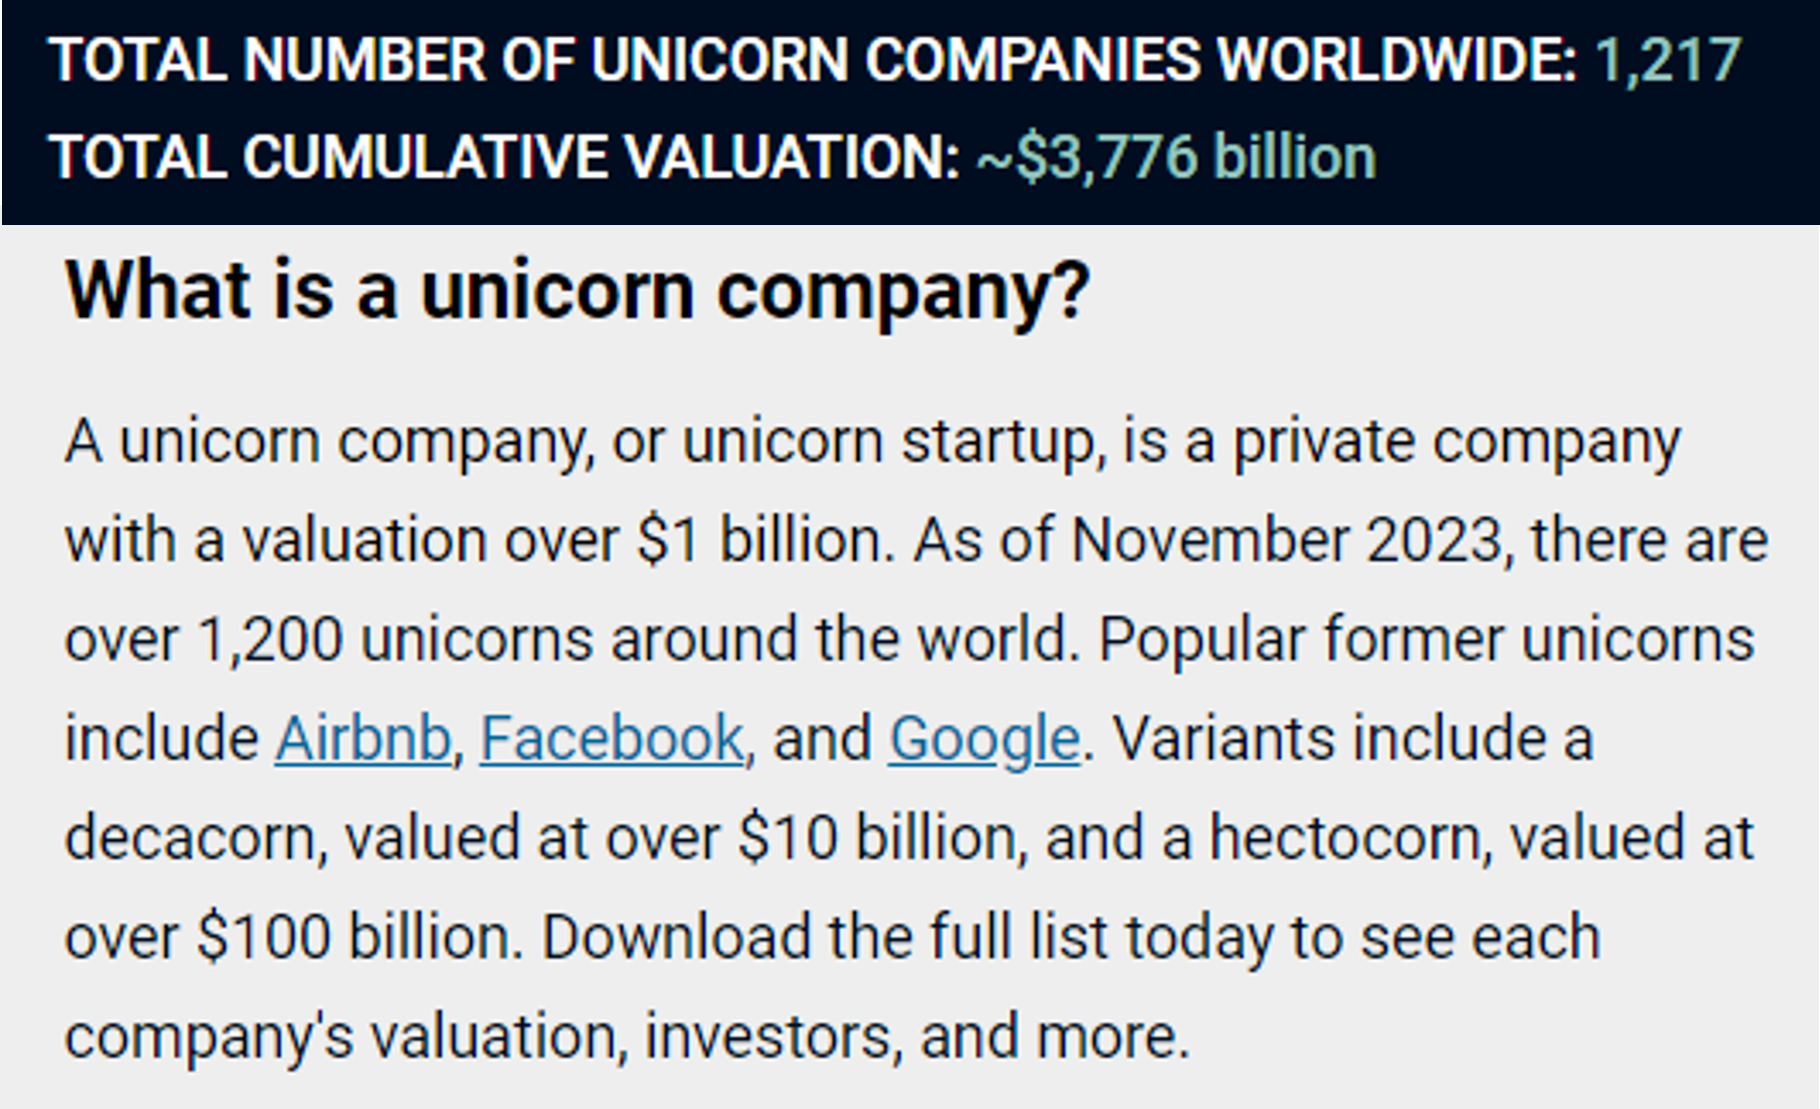
\includegraphics[]{pics/WhatIsUnicorn.png}
    } %end of resizebox
%-----------------------------------------------
% Figure setting: caption and label
%-----------------------------------------------
%\caption{Private Mortgages}
%\label{fig:ModelIntuition_Graphs}
\end{figure}
%-----------------------------------------------
\vspace{-2mm}

\href{https://www.cbinsights.com/research-unicorn-companies}{Source}

\end{frame} 
%----------------------------------------------------  


\begin{frame}{Stripe}

From payment processor Stripe's \href{https://assets.stripeassets.com/fzn2n1nzq965/2pt3yIHthraqR1KwXgr98U/df10795aac0205789956c89e0dfc4f1a/Stripe-annual-letter-2024.pdf}{annual letter: } 
\vfill 

``Businesses on Stripe generated \$1.4 trillion in total payment volume in 2024, up 38\% from the prior year, and reaching a scale equivalent to around 1.3\% of global GDP. We attribute this year’s rapid growth in part
to our long-standing investments in building machine learning and artificial intelligence into our products.'' 
\vfill 

\end{frame}

\begin{frame}{Stripe support for Agentic Workflow}

\begin{center}
    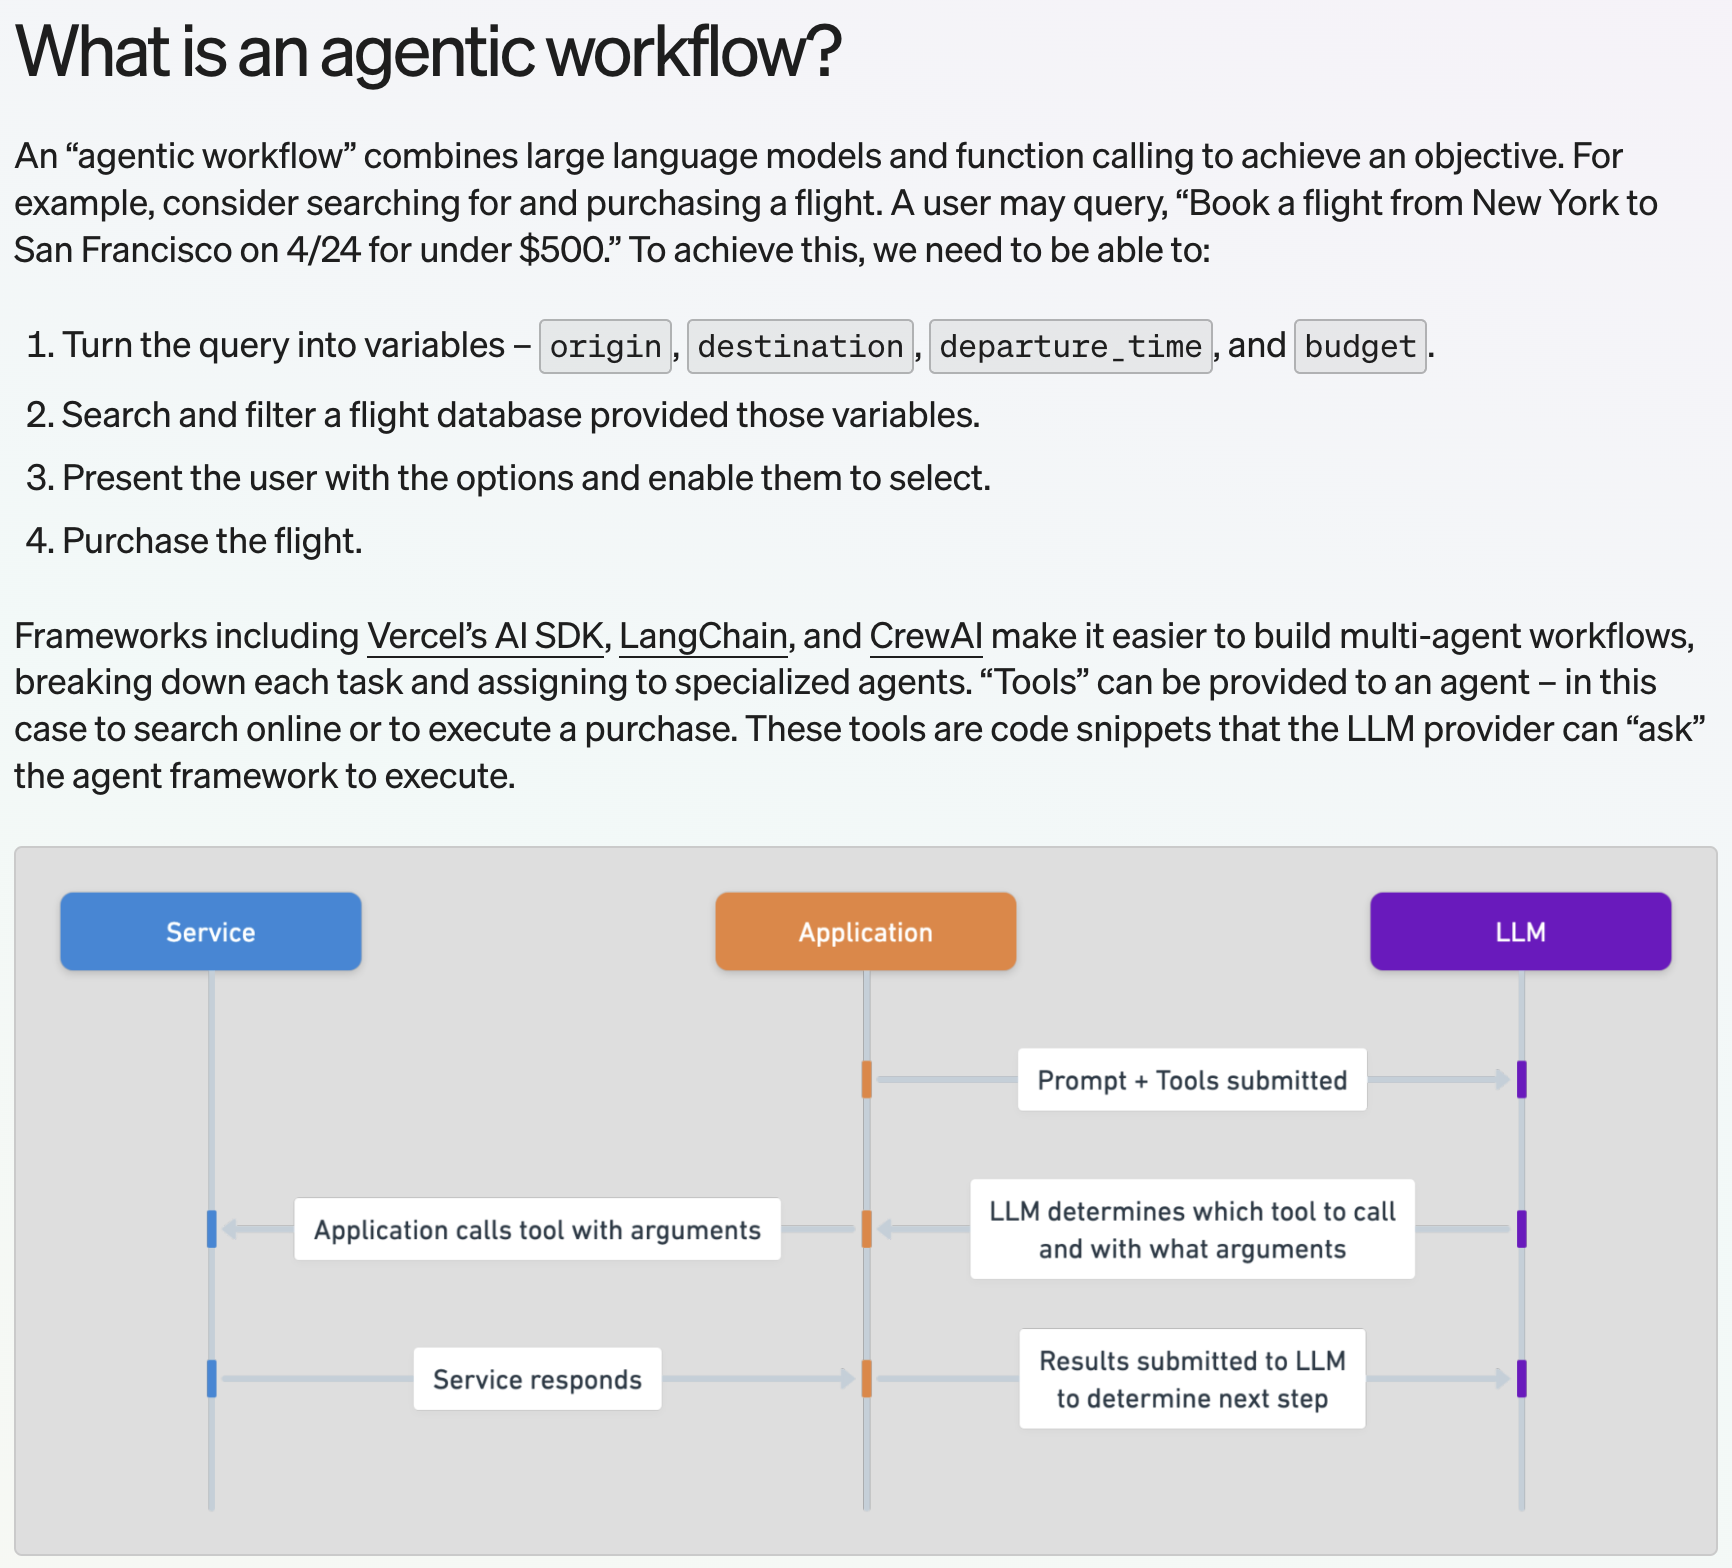
\includegraphics[height = .9\textheight]{agentic_workflow.png}
\end{center}

\end{frame}

\begin{frame}{Stripe API for AI agents}

\begin{center}
    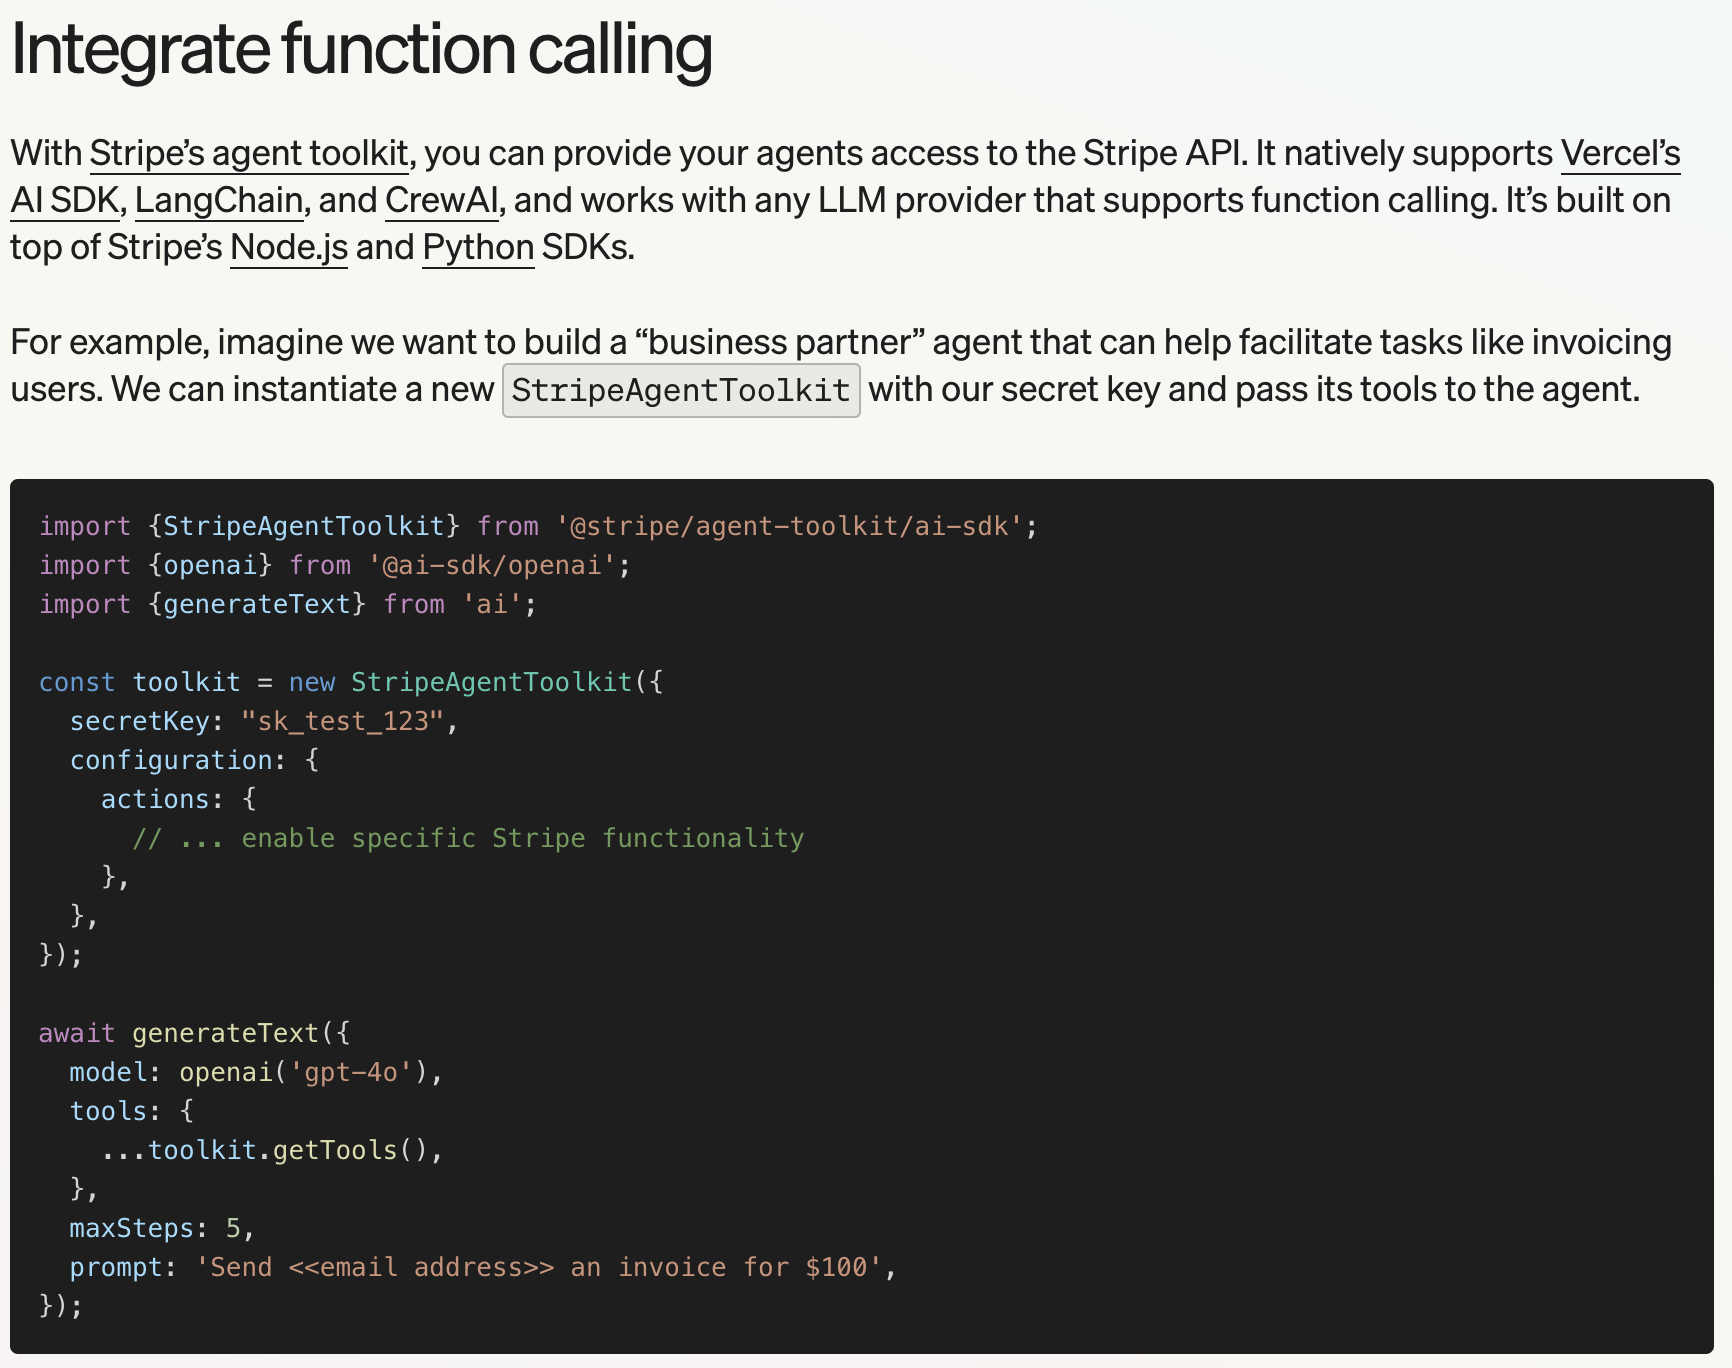
\includegraphics[height = .9\textheight]{integrate_function_calling.png}
\end{center}

\end{frame}

\begin{frame}{Give your AI agent a credit card}

\begin{center}
    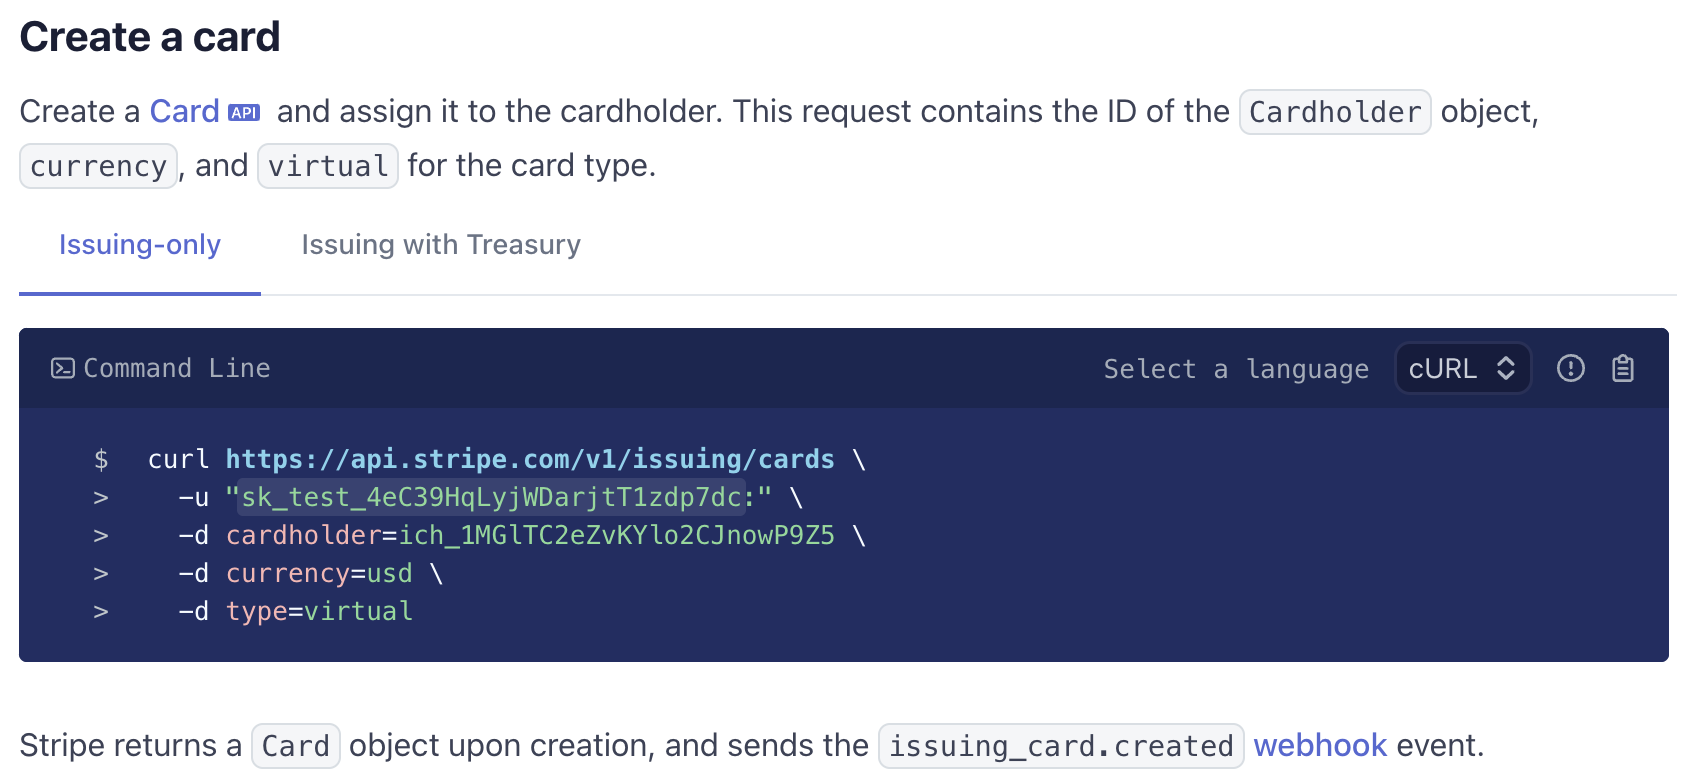
\includegraphics[width = \textwidth]{create_card.png}
\end{center}
\bi
\m A real human's name must still be on the credit card (why?) 
\ei 
    
\end{frame}

\begin{frame}{Stripe acquisition of Bridge}
\small  ``In October, we announced our acquisition of \href{https://www.bridge.xyz/}{Bridge}, the world’s leading stablecoin orchestration platform. Bridge enables businesses to do almost anything involving stablecoins: they make stablecoin-based applications easy to deploy and scale. They’re used by everyone from Scale AI to the world’s largest hodler [sic], the US government. \\
The top stablecoin use cases today involve tangible, real-world activity. CFOs use stablecoins to manage corporate treasury, immigrants use them for remittance, citizens of countries with unstable currencies use them for dependable savings, and payments teams use them to enable customers from countries with low card penetration. Some of our favorite examples: SpaceX uses Bridge to repatriate funds from Starlink sales in Argentina, Nigeria, and other markets. DolarApp, a neobank in Mexico, uses Bridge to help individuals receive USD payments from payroll providers like Deel. Airtm uses Bridge to disburse payments to workers all over Latin America.''
    
\end{frame}


\begin{frame}{Welcome! Today is Wednesday, October 29, 2025}

This is our third-to-last lecture of the semester! 
    
\end{frame}

\begin{frame}{Review: The Kelly Criterion}

From the quiz on Monday: what does the Kelly Criterion say to bet when offered +200 on a 50\% true probability event? \pause  \\ 

Edge is 50\%(3) - 1 = 0.5 \pause \\ 
Odds are 2 \pause \\ 
Edge / Odds = 0.5/2 = 25\% of your net worth. 
    
\end{frame}

\section{In the News}

\begin{frame}{Stablecoin Payments Jump 70\% Since New Regulation}

From Bloomberg via Matt Levine: \\

``Business-to-business transfers make up the most of stablecoin payments at \$6.4 billion monthly - nearly two-thirds of the total and up 113\% since February, the report said. This marks the first time business payments have exceeded peer-to-peer consumer transactions, which held steady at \$1.6 billion monthly, according to Artemis. Companies are using stablecoins to bypass traditional international banking delays.''
\\ \pause 
\bi 
\m Top use case: cross-border B2B payments where \textbf{settlement speed} is a priority 
\m \textbf{The total is still tiny} relative to bank-railed payments (70\% of a small number is small) 
\m 50\% of all currency moving to and from Venezuela is now in the form of Stablecoins, evading sanctions
\ei 

    
\end{frame}

\begin{frame}{Sports Dominate Prediction Markets}
\centering
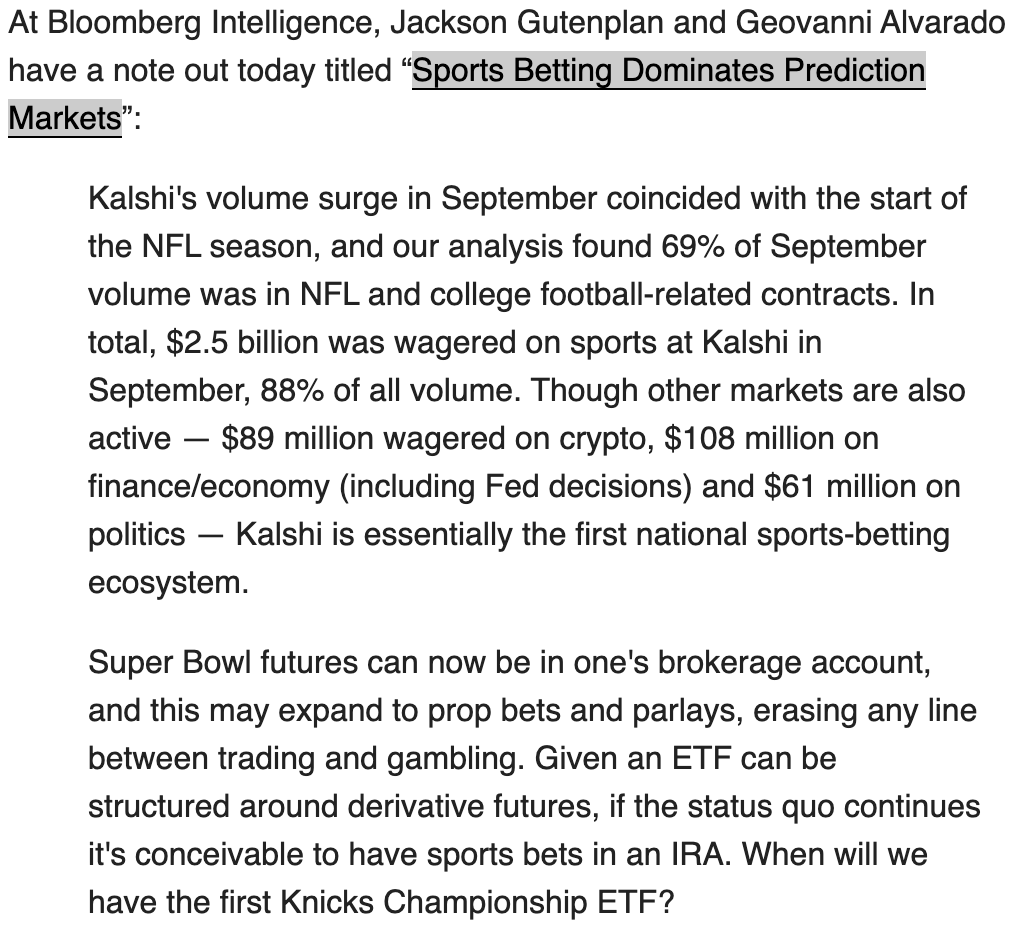
\includegraphics[height = .9\textheight]{matt_levine.png}
    
\end{frame}

\begin{frame}{Are Sports Prediction Markets Legal?}

\href{https://www.law.cornell.edu/cfr/text/17/40.11}{The law as written in the Code of Federal Regulations is awfully clear. No they are not!} \\ 

And yet, \textbf{prosecutorial discretion} is again the phrase of the day. \\ 

\begin{center}
    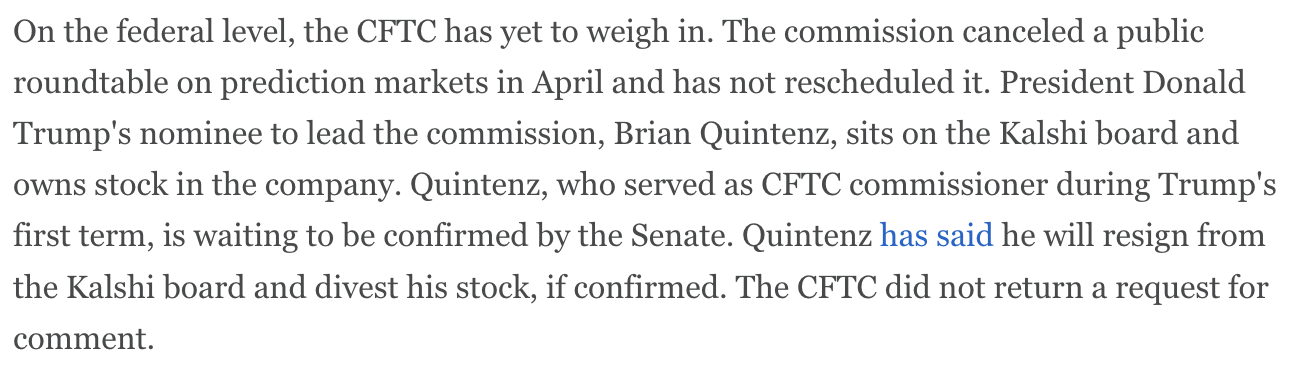
\includegraphics[width = .9\textwidth]{prosecutorial_discretion.png}
\end{center}
\pause 
Source: \href{https://www.espn.com/espn/betting/story/_/id/45377686/kalshi-prediction-markets-disrupt-sports-betting}{ESPN}
    
\end{frame}


\begin{frame}{Do Retail Prediction Markets Have a Legitimate Economic Purpose?}

\begin{center}
    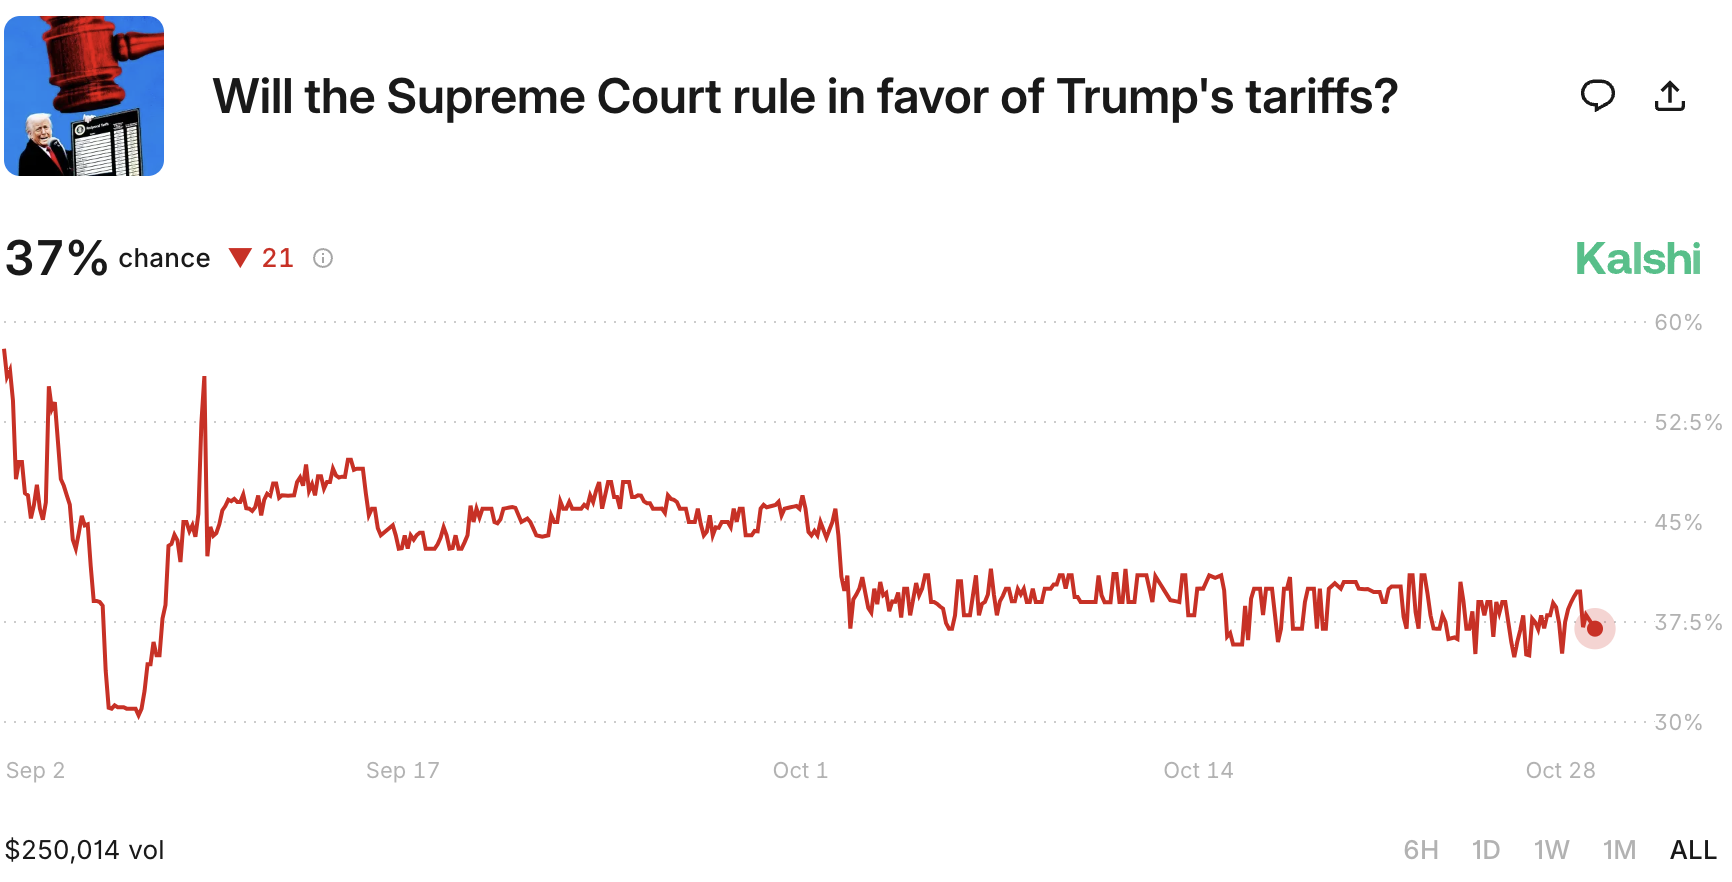
\includegraphics[width = \textwidth]{kalshi_tariffs.png}
\end{center}
    
\end{frame}

\begin{frame}{Are Retail Prediction Markets Good for Corporate Hedging?}

\bi 
\m Importers would love to hedge away tariff uncertainty \pause 
\m Only \$250,000 market depth on Kalshi -- could a corporate importer drop \$1 million into this market? 
\pause 
\bi 
\m Absolutely not. 
\ei 
\m Importers are doing this trade, but not on a retail exchange: Jefferies, Oppenheimer among Wall Street banks writing ``tariff insurance'' for corporates, some \emph{over \$100 million} notional \\ 
\m Does this mean Kalshi is useless? \pause Not necessarily! Kalshi provides a publicly-available \textbf{reference price} for these privately-negotiated contracts
\bi 
\m The provision of \textbf{reference prices} in financial markets is extremely important, especially when they are prone to manipulation! See, for instance, how major banks recently started indexing contracts to the \href{https://www.newyorkfed.org/markets/reference-rates/sofr}{SOFR reference rate}, instead of LIBOR, precisely because SOFR is a public market price (unlike LIBOR) 
\ei 
\ei 
    
\end{frame}


\section{Fast Payment Blockchains}

\begin{frame}{Corporate Blockchains}

Recall when we discussed the \textbf{decentralization trade-off}: a decentralized system requires \emph{redundancy} to be trustless, and this redundancy is very computationally expensive. Corporate blockchains (AKA ``permissioned'', ``private'', ``high-throughput'', or ``performance'') blockchains dispense with trustlessness to prioritize speed above all. \\ \pause 
At least three large projects aim to become the base layer for global payments: 

\bi 
\m \textbf{Stripe} (enterprise payments provider) has acquired the \href{https://www.bridge.xyz/}{Bridge} platform (more like a UI/SAAS for businesses) and the \href{https://tempo.xyz/}{Tempo} blockchain 
\m \textbf{Tether} (\#1 stablecoin issuer) is affiliated with \textbf{Plasma}
\m \textbf{Circle} (\#2 stablecoin issuer) is building \textbf{Arc} (which we discussed recently) 
\ei 

\pause 
Each of these projects promises Real-Time Gross Settlement on the order of milliseconds and relies on regulated Stablecoins as medium of exchange. 


\end{frame}


\begin{frame}{Advantages of Fast Payment Blockchains}

If decentralization is abandoned as a goal, why even encode payments on a blockchain instead of just a trusted database? \\ \pause 
Some advantages of Blockchain technology remain despite losing decentralization: 

\bi 
\m \textbf{Smart Contracts} can run verifiably on private blockchains (subject to censorship -- but not manipulation, as we discussed earlier) 
\m \textbf{Digital Signatures} create tamper-proof records 
\m \textbf{Customizable Privacy} can allow users to toggle and verifiably control their level of anonymity (a priority for, e.g., Arc) \pause 
\ei 
However, serious criticisms remain that a corporate-controlled, government-controlled system will deliver competitive prices and guarantees against censorship and inflation: \href{https://malekanoms.substack.com/p/corporate-blockchains-are-unlikely}{Omed Malekan}


    
\end{frame}


\begin{frame}{Smart Contract Use Case for Corporate Blockchains: FX Trade}

\begin{center}
    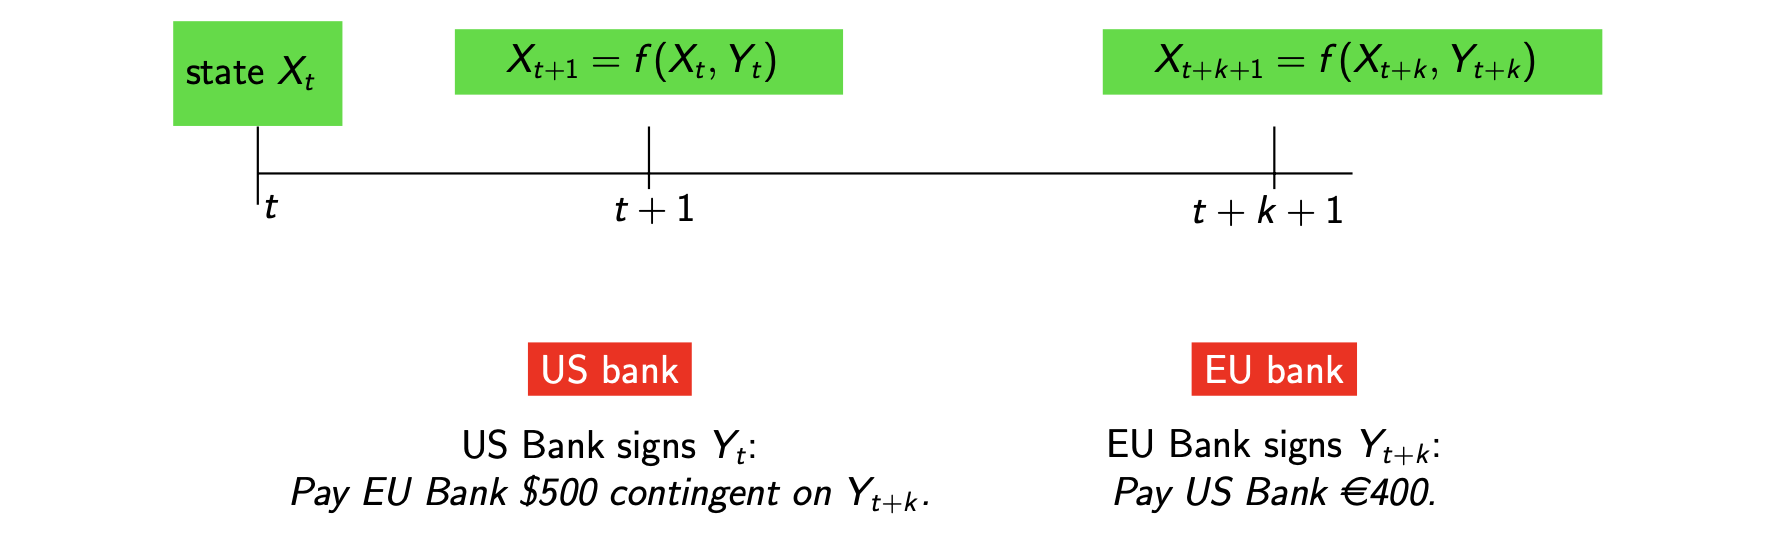
\includegraphics[width = \textwidth]{duffie.png}
\end{center}

\bi 
\m Blockchains allow \emph{contingent transfers} without trusting the counterparty or even a clearinghouse (Graphics by Darrell Duffie) 
\m \href{https://www.bis.org/about/bisih/topics/cbdc/jura.htm}{Jura} (France and Switzerland), \href{https://www.newyorkfed.org/medialibrary/media/nyic/project-cedar-phase-two-ubin-report.pdf}{Cedar} (FRBNY + Singapore) 
\ei 
    
\end{frame}

\begin{frame}{Projected Growth of Stablecoins}

\begin{center}
    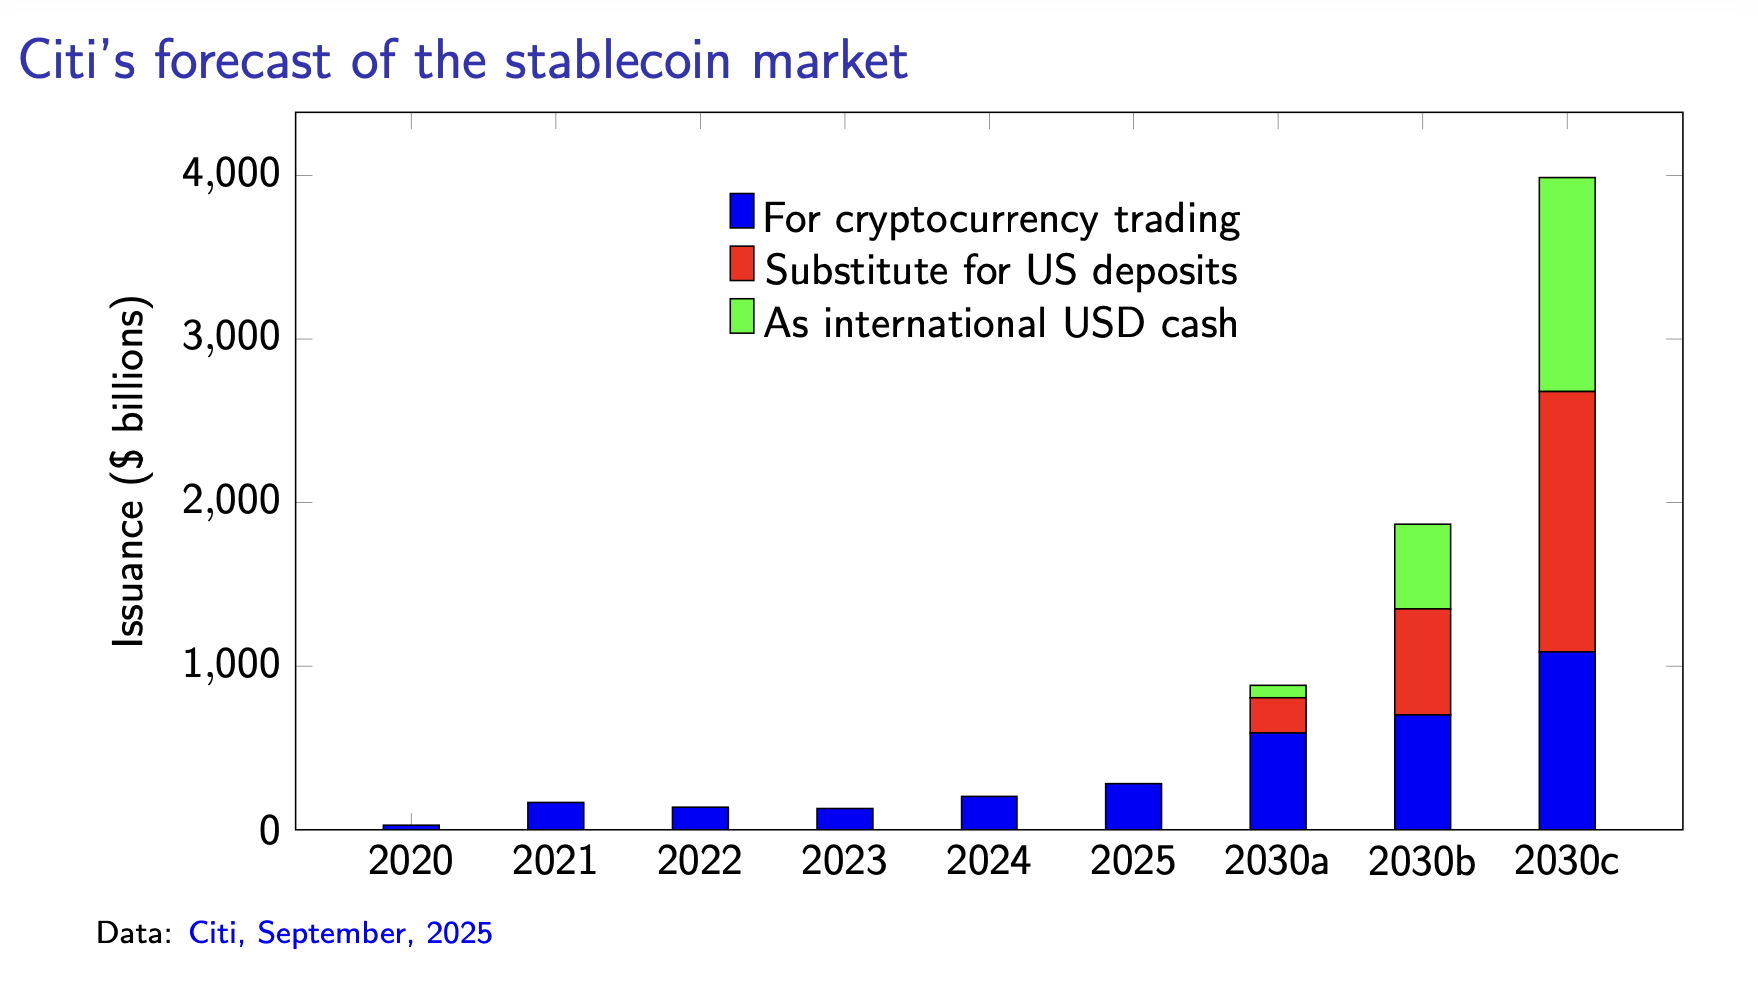
\includegraphics[width = .95\textwidth]{duffie_2.png}
\end{center}
    
\end{frame}


\begin{frame}{Macroeconomic Concerns}

A number of macroeonomic concerns have been raised around the possibility of corporate stablecoins displacing traditional payment rails: 

\bi 
\m \textbf{Excessive Leverage}: Stablecoin issuers may over-mint, make bad investments, or be run on 
\m \textbf{Loss of Credit Supply}: If traditional banks lose deposits they may make fewer loans, harming growth 
\ei 

My opinions: Critique 1 is weak because Stablecoin issuers will be no harder to regulate macroprudentially than banks (they may in fact be much easier to regulate) in the long run.  My response to critique 2 is that consumers should have the choice to hold cash-like, non-interest-bearing digital assets without them being secretly lent out. \\ 
\bi 
\m These are the exact same concerns the United States faced with private banknotes in the Free Banking Era (1863 to 1935)! 
\ei 
    
\end{frame}

\begin{frame}{Ye Olde StableCoins}
\centering 
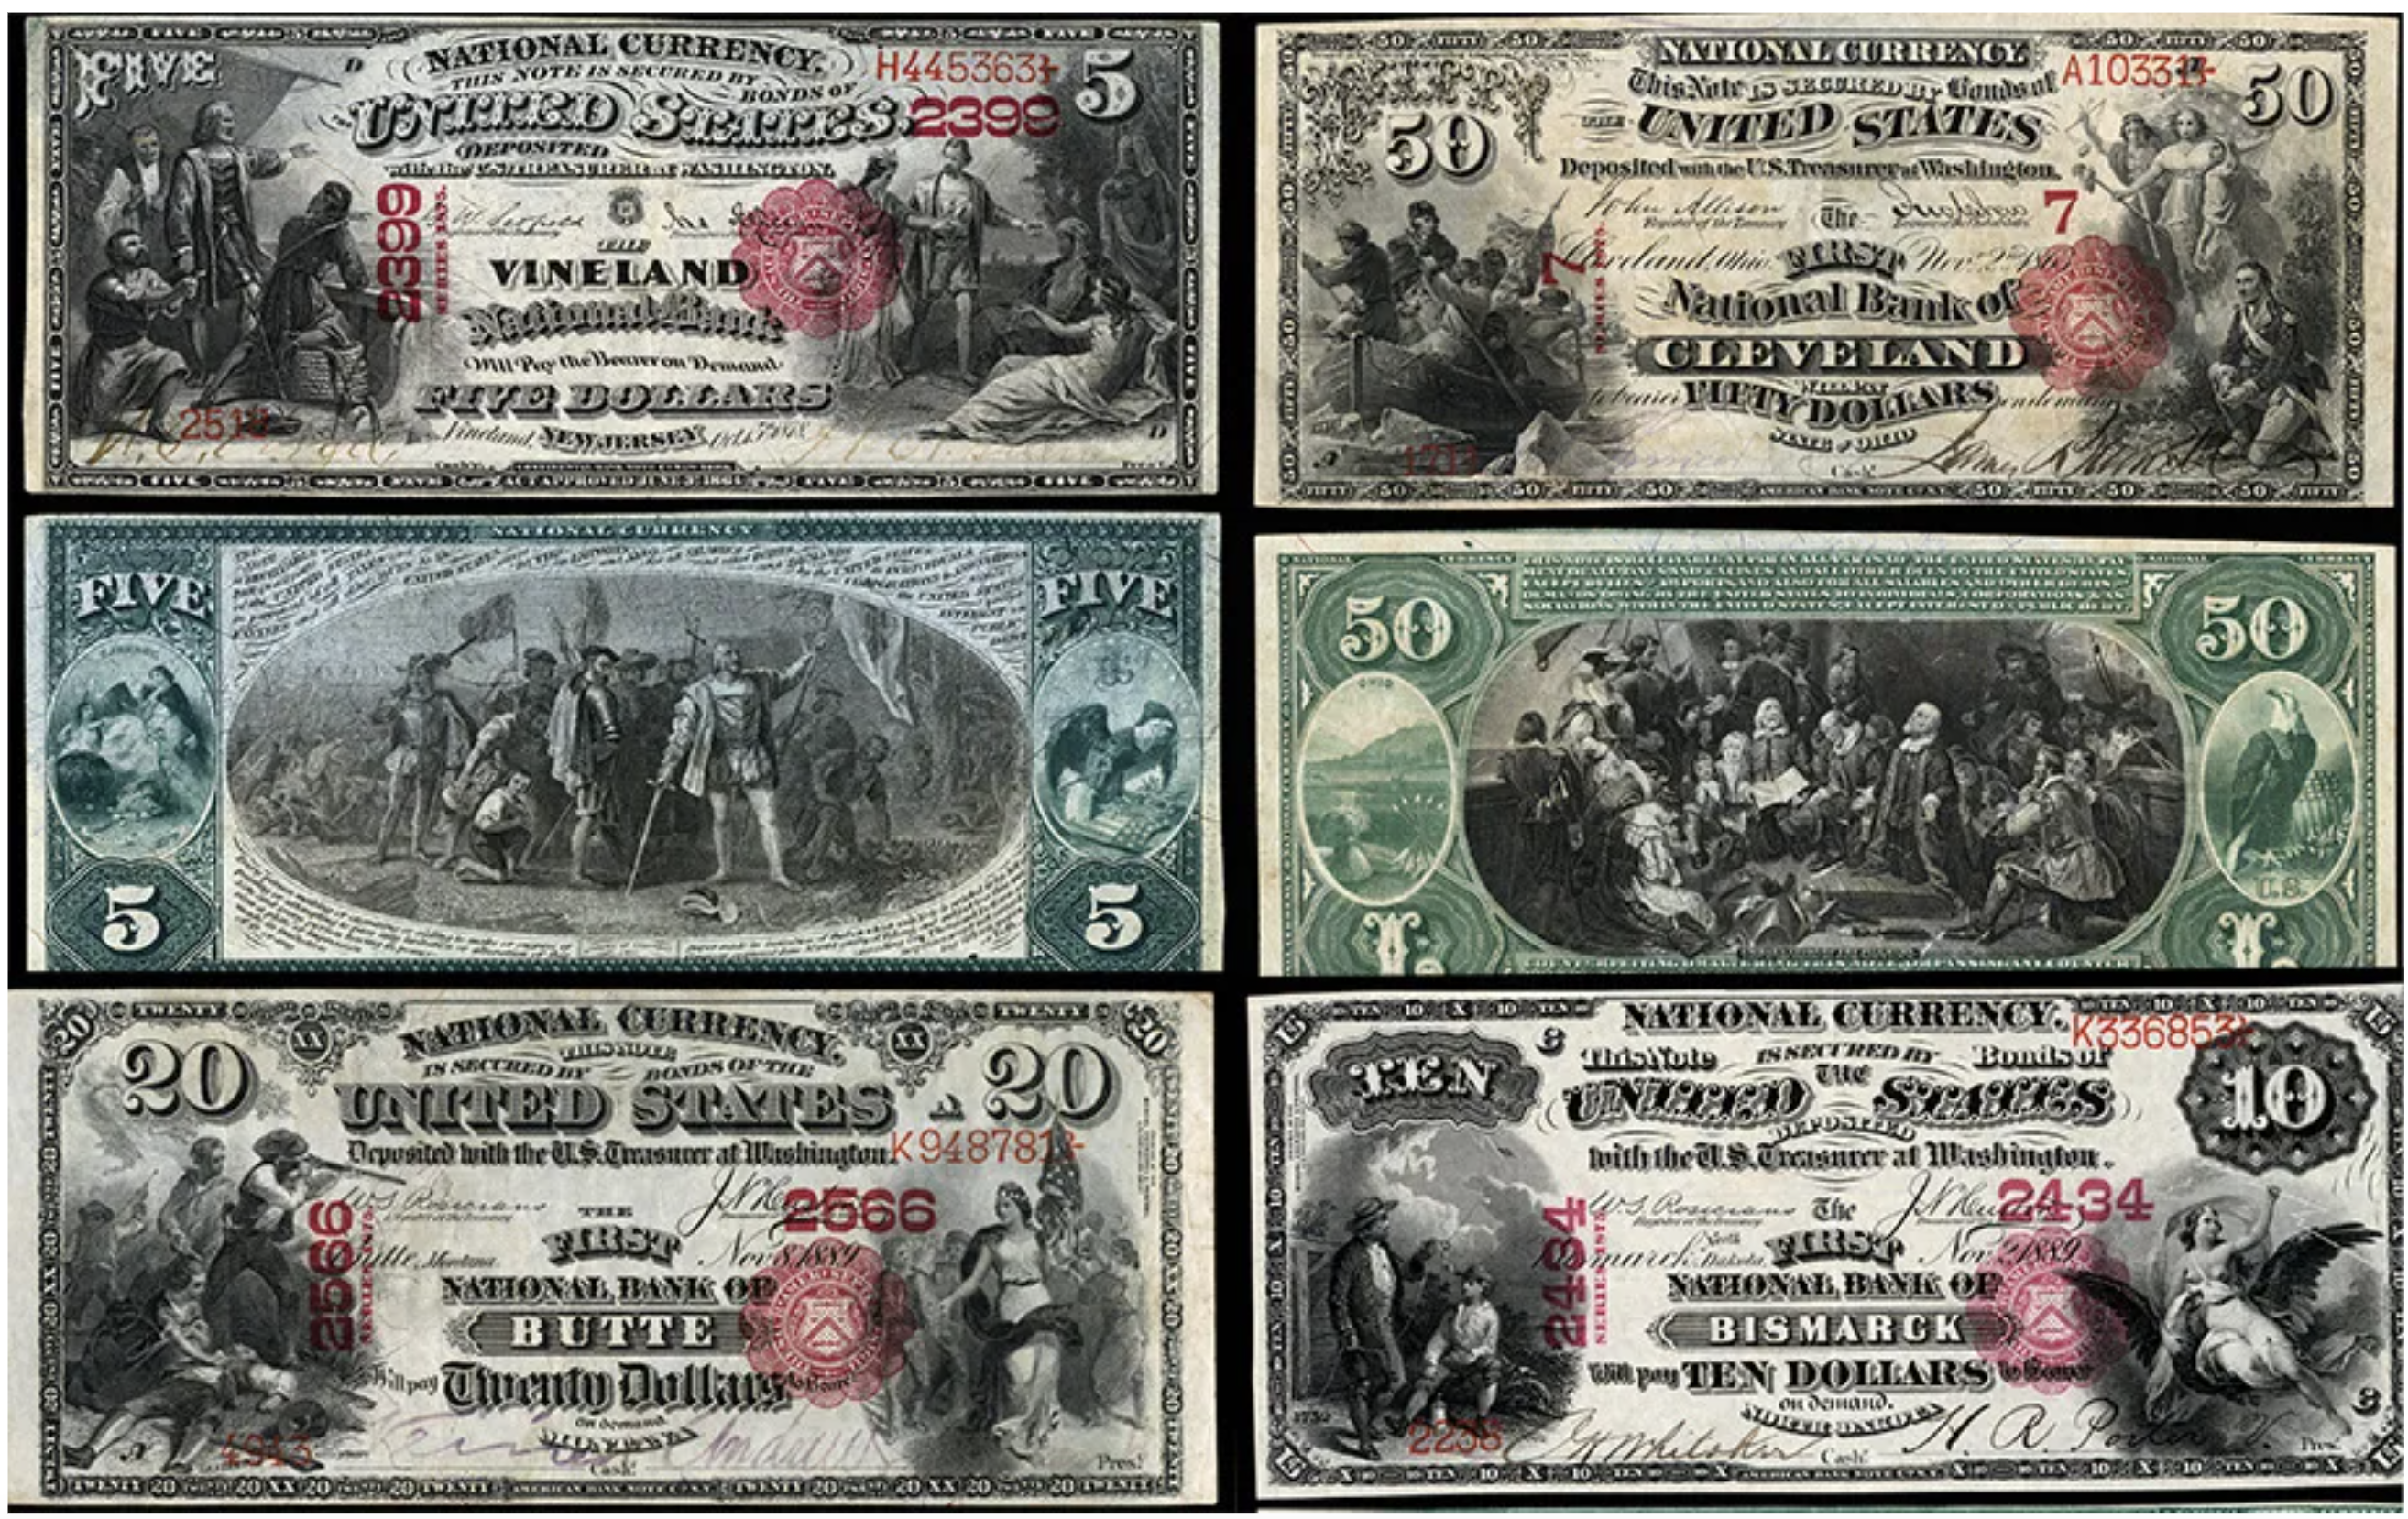
\includegraphics[height = .9\textheight]{ye_olde_stablecoins.png}
    
\end{frame}

\begin{frame}{Free Banking Era vs. Modern ``Stablecoin Era''}

The Free Banking Era ended with a disastrous economic collapse. Have we learned our lesson? \\ 

\bi 
\m \textbf{Collateral Requirements}: FBA allowed state-issued bonds to be used as collateral, which frequently defaulted! GENIUS Act only allows federal bonds as collateral in U.S.. 
\m \textbf{Fungibility}: Lack of fungibility between banknotes hindered their ability to function as money. This concern is particularly strong today in Europe, which lacks fiscal unity $\rightarrow$ e.g. Greek stablecoins might not trade at par with German ones. 
\m \textbf{Seignorage}: Banks collected interest on bonds while issuing interest-free notes (or today, stablecoins), allowing them to capture \emph{seignorage} instead of the federal government! This can weaken the financial position of the U.S. Treasury. 
\ei 

Source: \href{https://libertystreeteconomics.newyorkfed.org/2025/10/a-historical-perspective-on-stablecoins/}{Stephan Luck, FRBNY for Liberty Street Economics}
    
\end{frame}




\section{Credit Cards}

\begin{frame}{Credit Cards Dominate U.S. Payments}

\begin{center}
    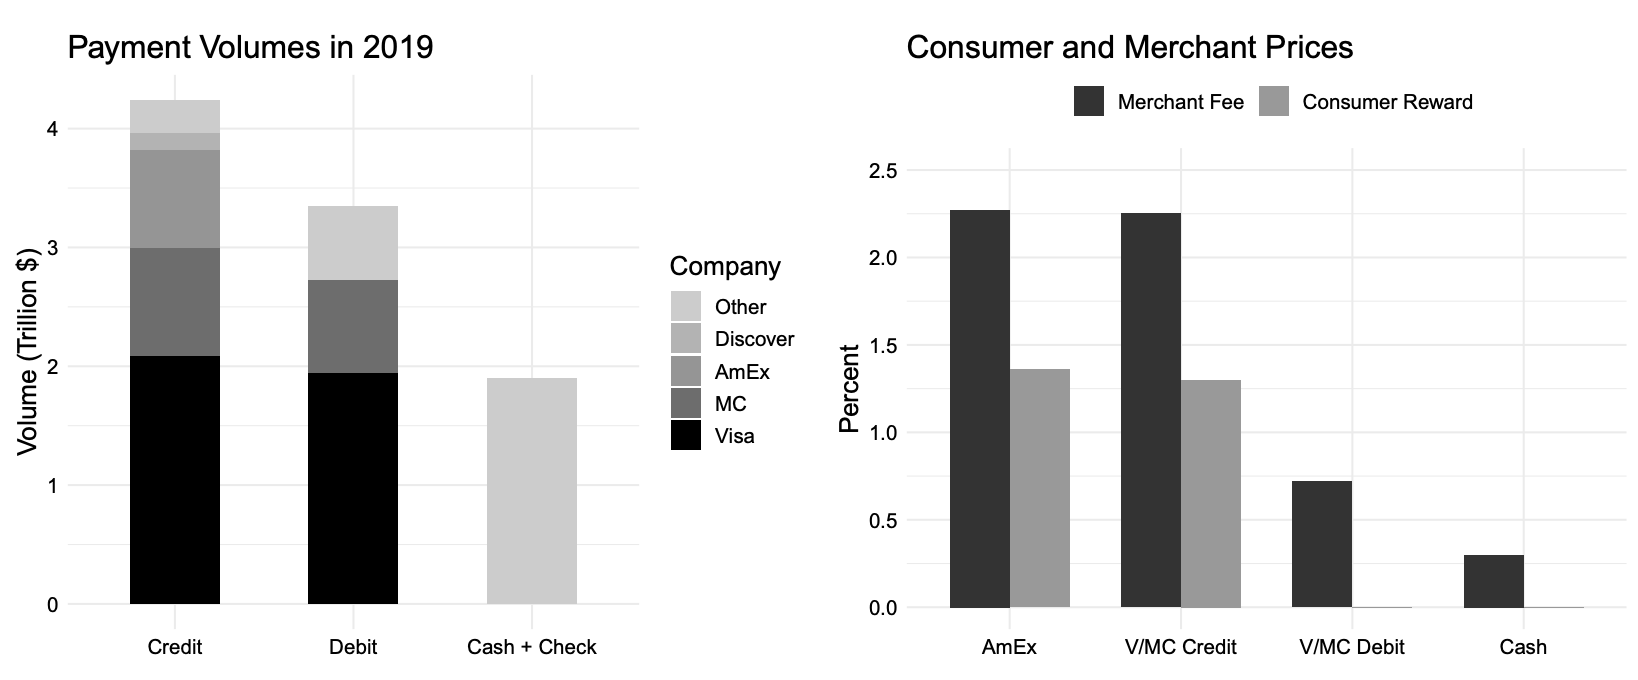
\includegraphics[width = .9\textwidth]{wang_1.png}
\end{center}
Source: \href{https://luluywang.github.io/PaperRepository/payment_jmp.pdf}{Lulu Y. Wang, Kellogg SOM}
    
\end{frame}




\begin{frame}{Credit Cards Bundle Payments and Lending}

\bi 
\m A Credit Card is not just a payment, but also a revolving loan that starts incurring interest if it is not repaid at the end of the month following the purchase 
\m Why are credit cards so popular relative to debit cards in the U.S.?\pause  
\bi 
\m Americans are impatient and optimistic, so we just love to borrow (Hall (2025)) \pause 
\m The \textbf{Durbin Amendment} caps interchange fees for debit cards but not for credit cards $\rightarrow$ banks steer customers towards using cards to collect more fees from merchants (Wang (2024))
\m Merchants are increasingly \textbf{surcharging} to equalize these fees and make cardholders internalize the card fee, but cardholders continue to perceive this as an \emph{unfair business practice}, harming brand value of merchants who do surcharge. 
\ei 
\m Creditworthy customers are also more profitable customers for businesses! Merchants pay interchange for \emph{access} to high-margin customer flow. Would you rather fill up your store with Low-FICO or High-FICO customers? 
\ei 
    
\end{frame}




\begin{frame}{Credit Cards Comprise Two Parallel Economies}

The economics of High- and Low-FICO (credit score) credit cards are totally different, despite using the same type of contract! \\ 

\textbf{Cost Side} (from bank's perspective)
\bi
\m \textbf{High FICO}: High volume but low default rate: cost is \textbf{rewards expenses} (paying to give cardholders AmEx Lounges etc.) 
\m \textbf{Low FICO}: Low volume but high default rate: cost is \textbf{chargeoffs} (loan not paid and no collateral) 
\ei 

\textbf{Revenue Side} (from bank's perspective)
\bi
\m \textbf{High FICO}: High volume = high \textbf{interchange income}
\bi
\m Banks can demand higher fees from merchants to process payments from richer, more profitable customers 
\ei 
\m \textbf{Low FICO}: Keeping high balances, and not paying off in full, for many months means means high \textbf{interest and fee income}
\ei 
    
\end{frame}

\begin{frame}{Credit Cards Comprise Two Parallel Economics}

In summary: 

\bi
\m \textbf{low-FICO} credit cards are a lending business comparable to payday loans. 
\m \textbf{high-FICO} credit cards are a utility and service business comparable to subscriptions.
\ei 
    
\end{frame}


\begin{frame}
\frametitle{Credit Card Payment Infrastructure: Fees}

\vspace{-4mm}
%-----------------------------------------------
\begin{figure}[H]
    \resizebox{5.4in}{2.4in}{%
    %\resizebox{\textwidth}{!}{%
    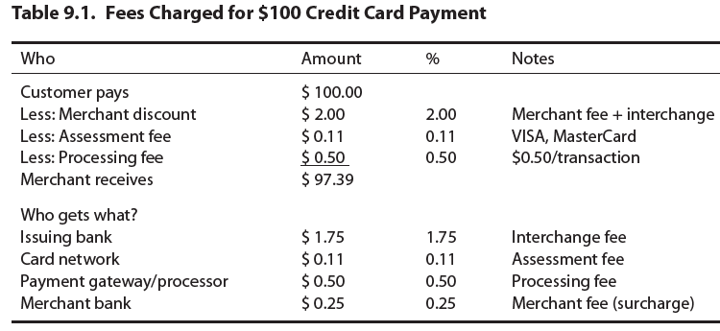
\includegraphics[]{pics/CreditCardPaymentInFees.png}
    } %end of resizebox
%-----------------------------------------------
% Figure setting: caption and label
%-----------------------------------------------
%\caption{Private Mortgages}
%\label{fig:ModelIntuition_Graphs}
\end{figure}
%-----------------------------------------------
\vspace{-2mm}


\end{frame} 
%----------------------------------------------------  


\begin{frame}{Credit Card Payment Flowchart}
\begin{center}
       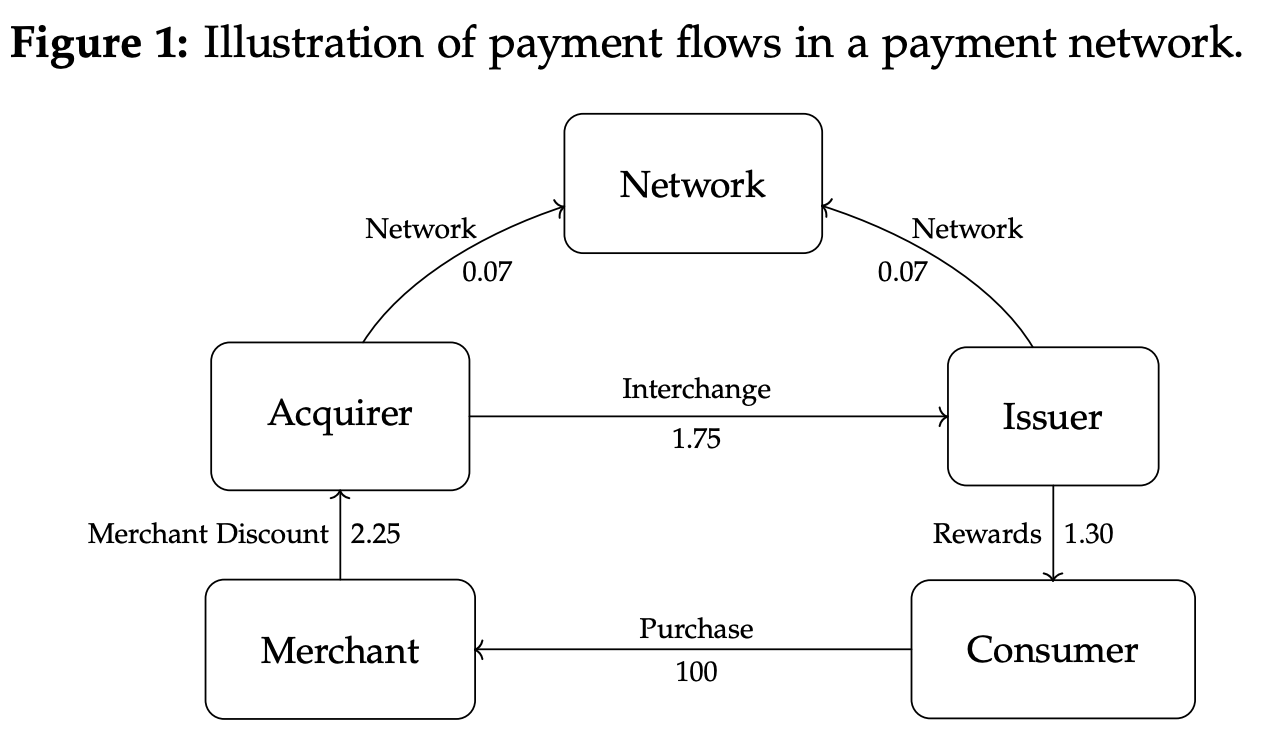
\includegraphics[width = .8\textwidth]{paymet_flows.png} 
\end{center}
Wang (2024) 
\end{frame}


\begin{frame}{Credit Cards Comprise Two Parallel Economies}

\begin{center}
    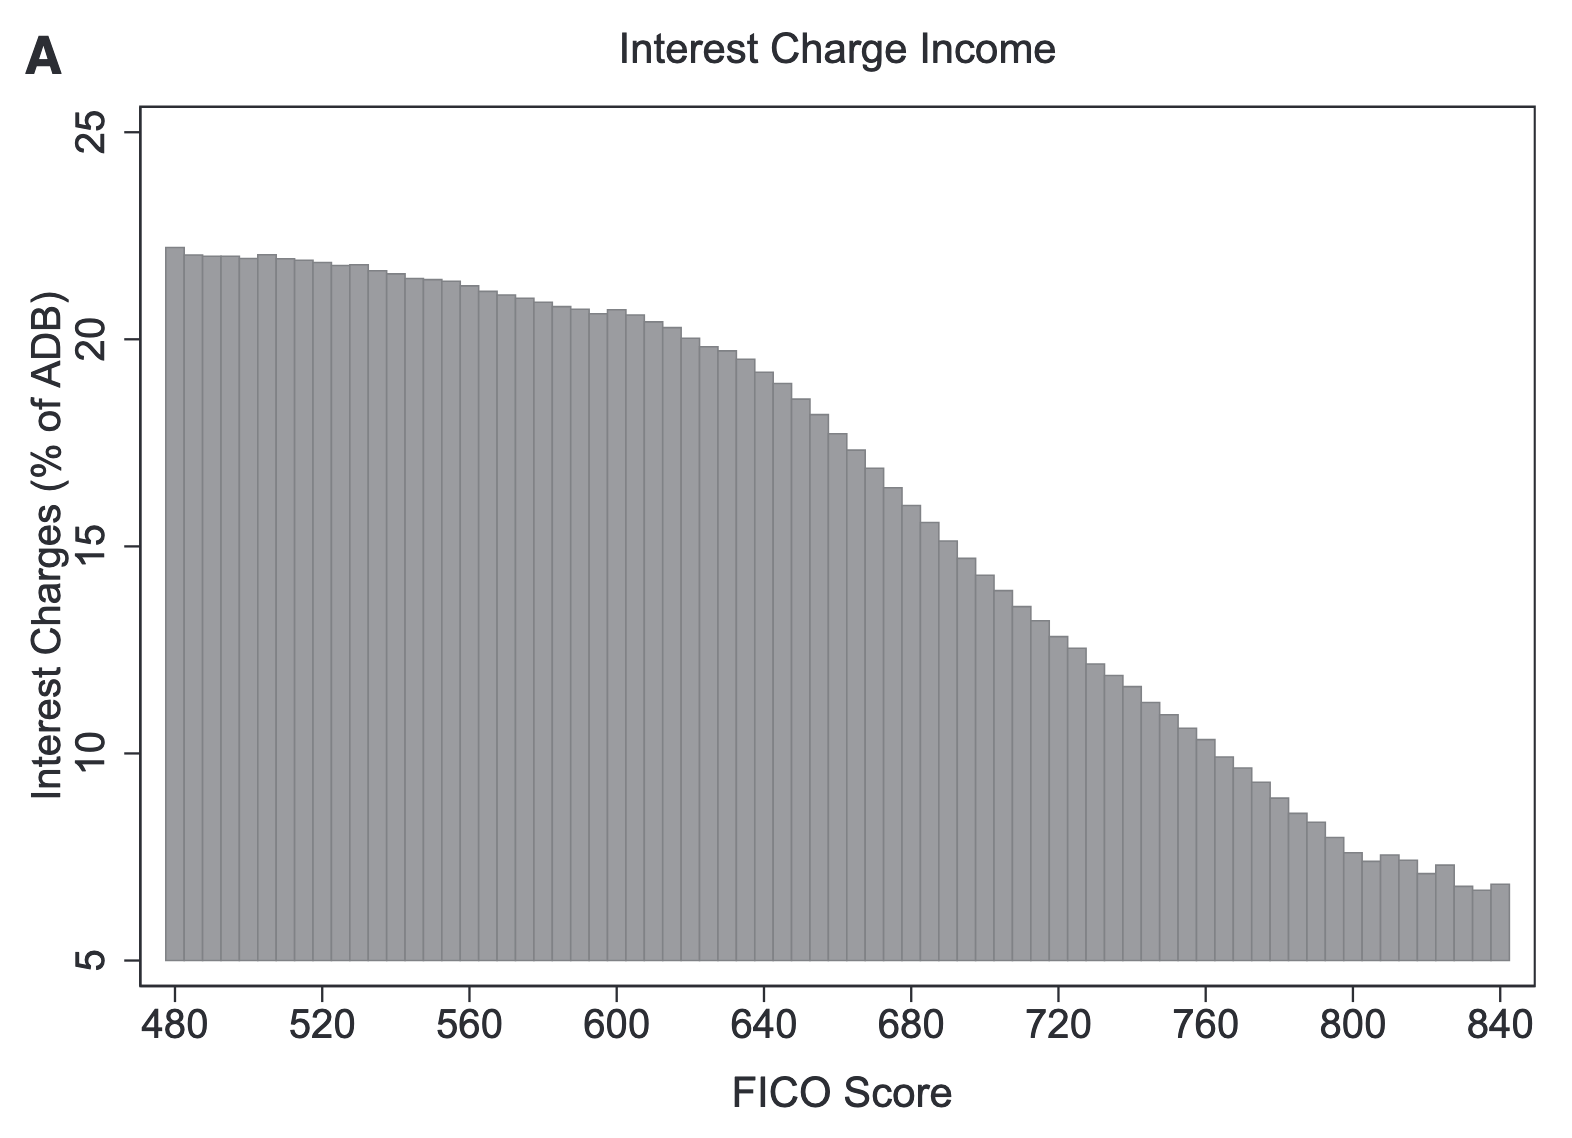
\includegraphics[width = .6\textwidth]{panel_a.png}
\end{center}
    
\end{frame}

\begin{frame}{Credit Cards Comprise Two Parallel Economies}

\begin{center}
    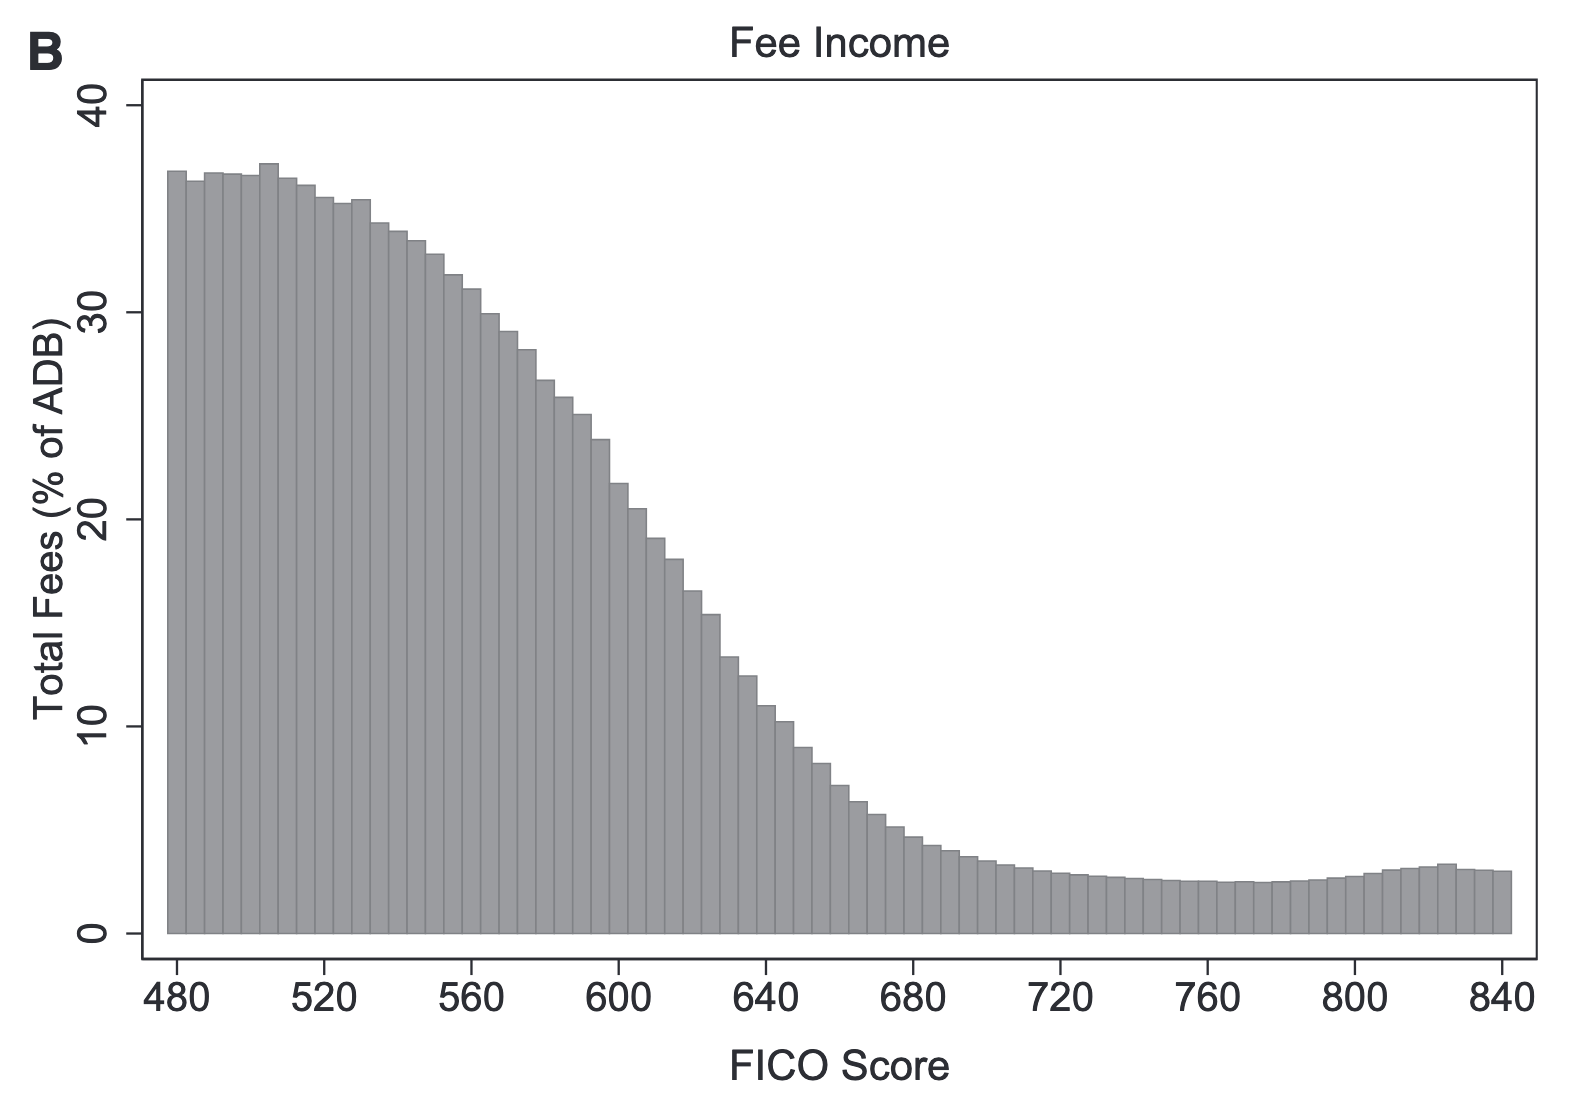
\includegraphics[width = .6\textwidth]{panel_b.png}
\end{center}
    
\end{frame}

\begin{frame}{Credit Cards Comprise Two Parallel Economies}

\begin{center}
    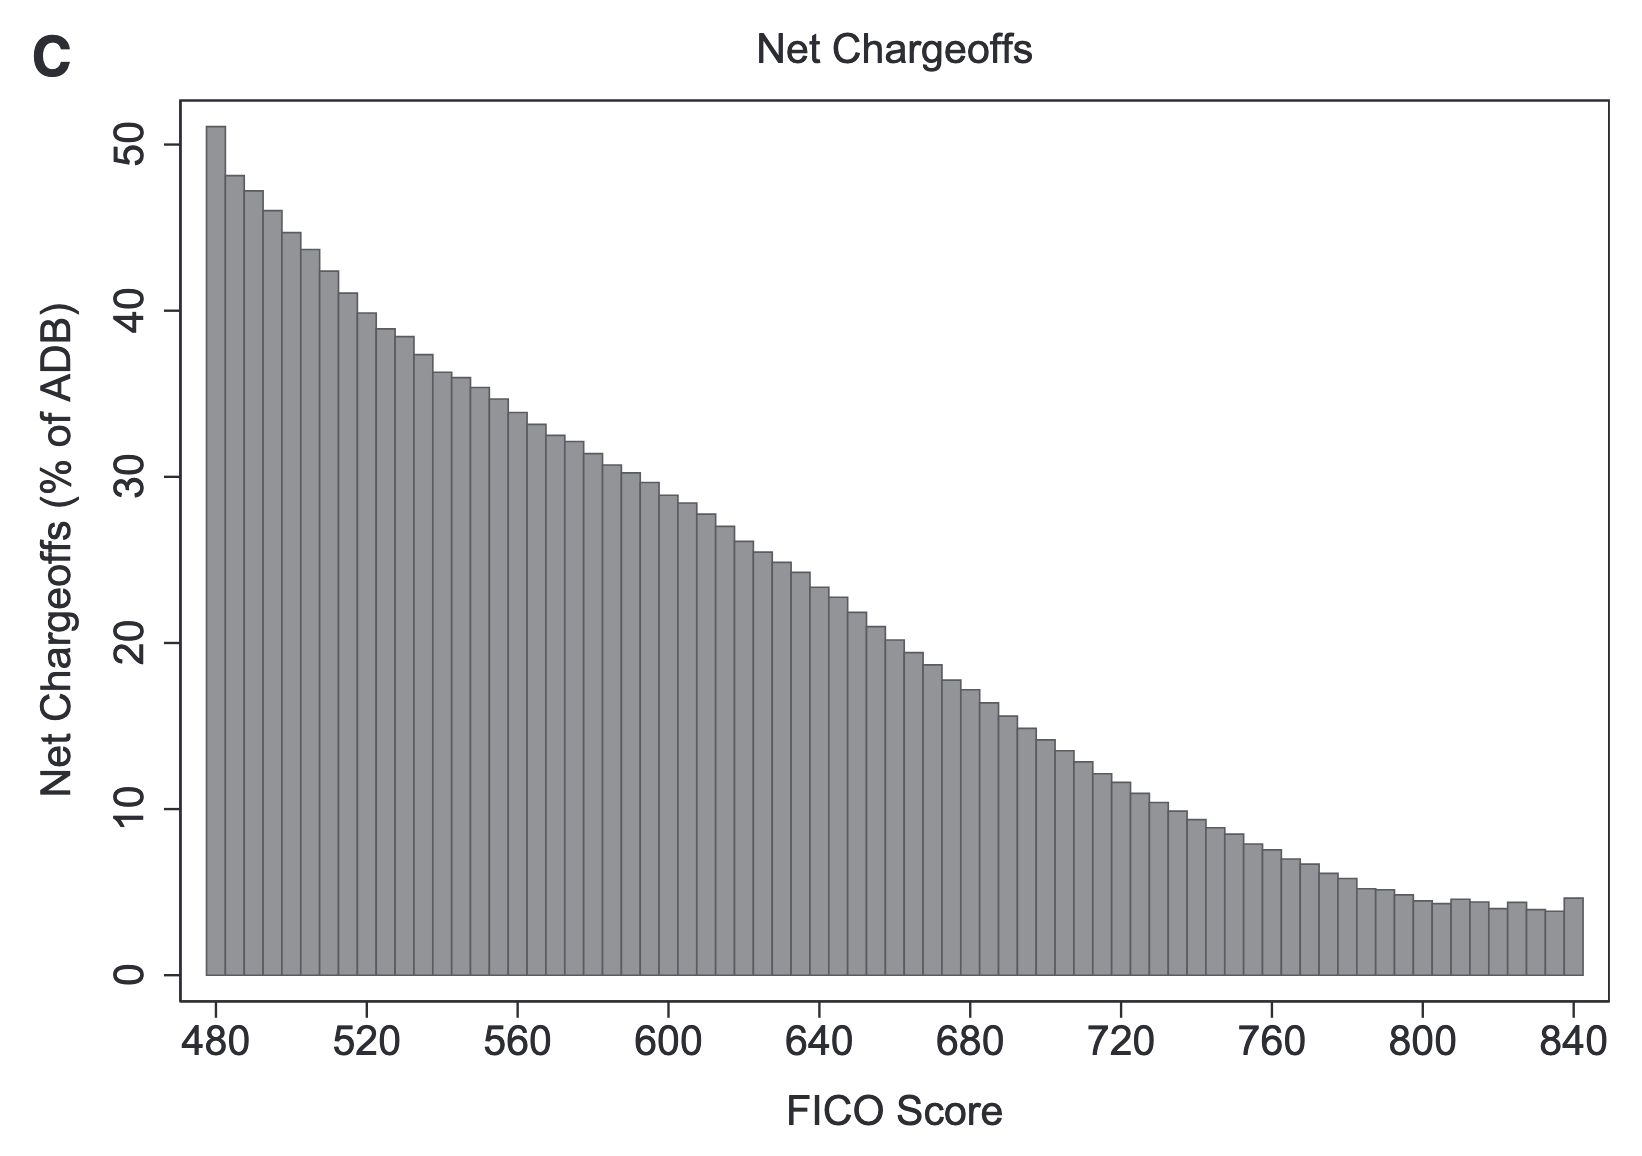
\includegraphics[width = .6\textwidth]{panel_c.png}
\end{center}
    
\end{frame}
\begin{frame}{Credit Cards Comprise Two Parallel Economies}

\begin{center}
    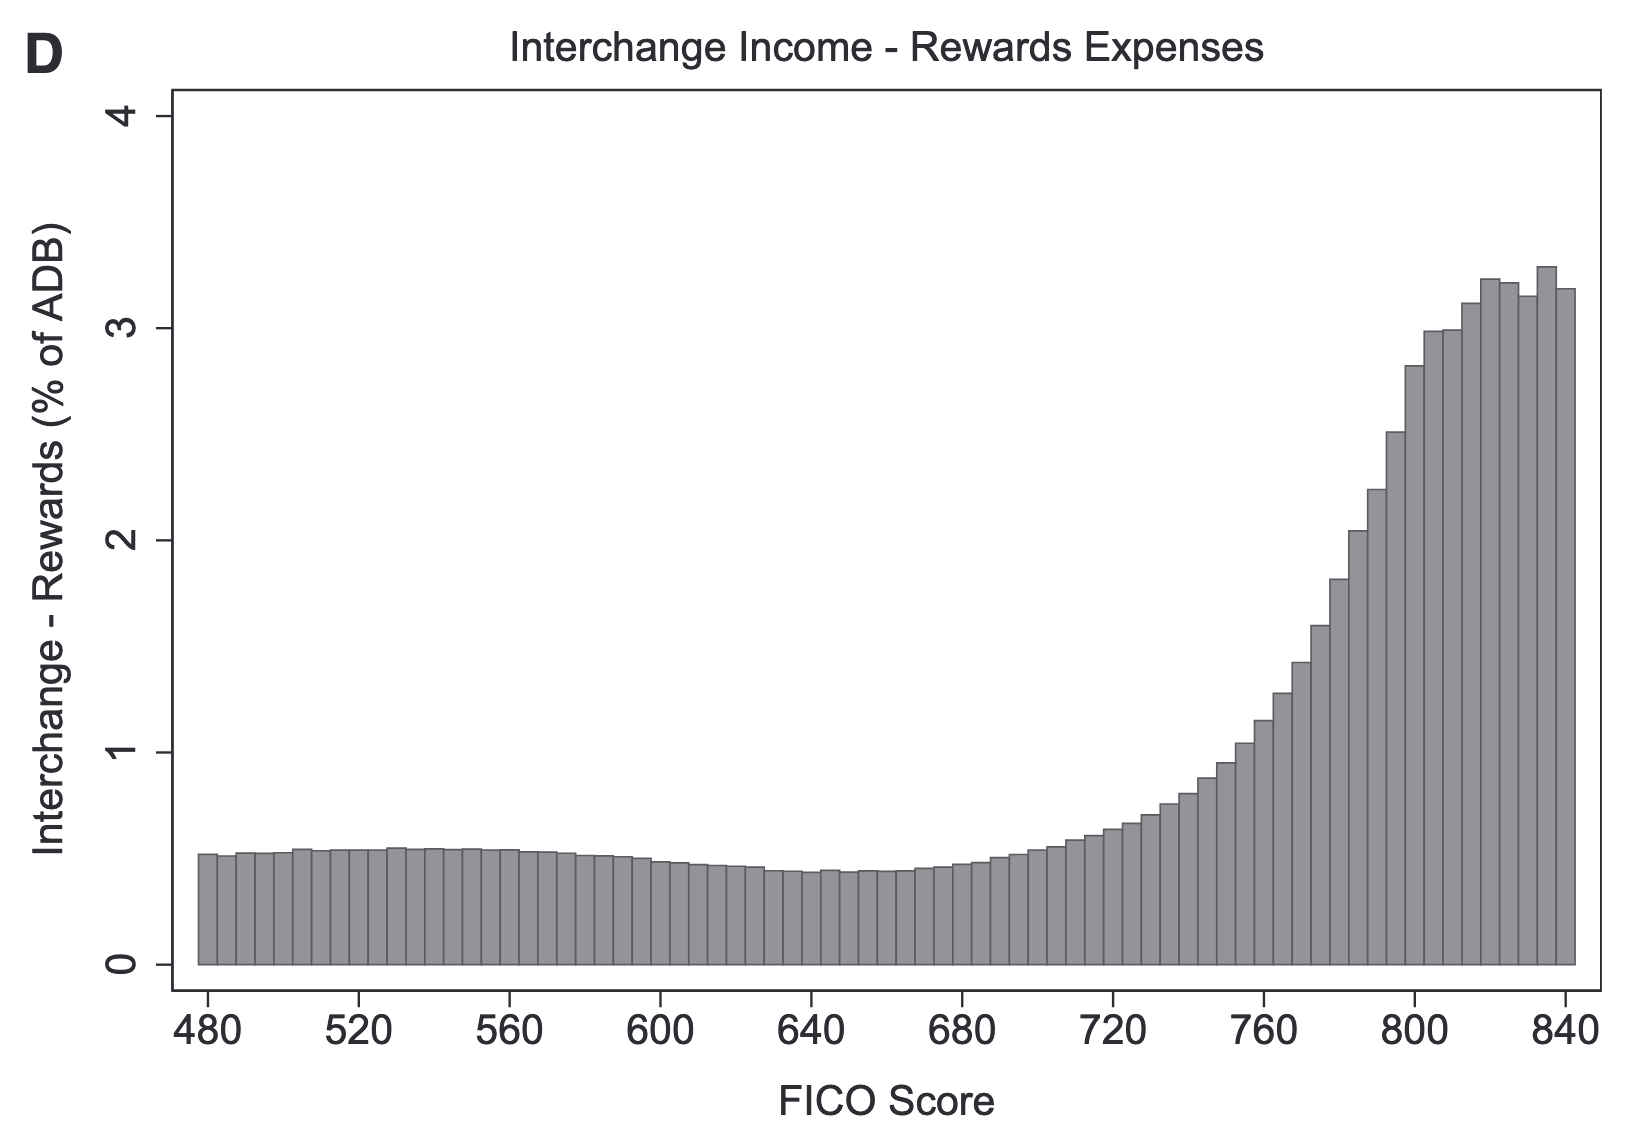
\includegraphics[width = .6\textwidth]{panel_d.png}
\end{center}
    
\end{frame}
\begin{frame}{Credit Cards Comprise Two Parallel Economies}

\begin{center}
    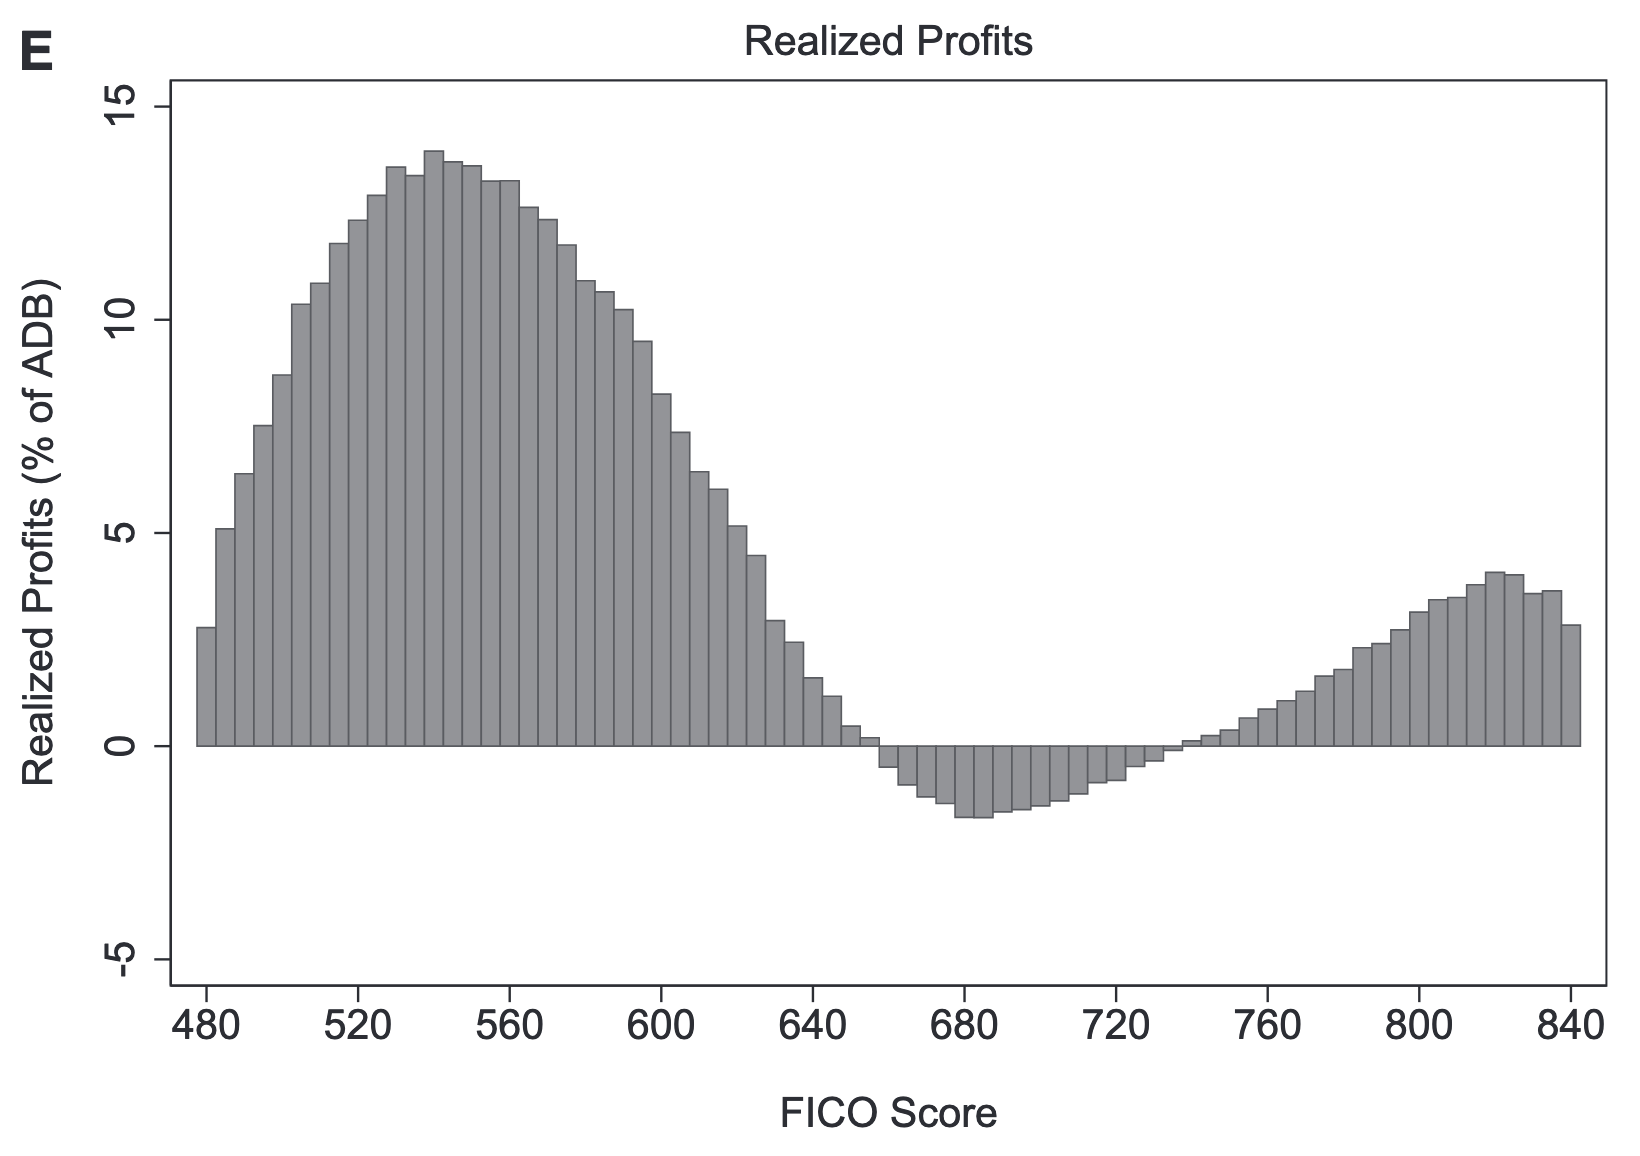
\includegraphics[width = .6\textwidth]{panel_e.png}
\end{center}
Source: \href{https://www.nber.org/papers/w19484}{Agarwal et al (2015)}
\end{frame}




\end{document}